%% LyX 2.1.1 created this file.  For more info, see http://www.lyx.org/.
%% Do not edit unless you really know what you are doing.
\documentclass[12pt,english,mathserif, professionalfonts]{beamer}
\usepackage{mathpazo}
\usepackage[T1]{fontenc}
\usepackage[latin9]{inputenc}
\usepackage{units}
\usepackage{bm}
\usepackage{amsmath}
\usepackage{amssymb}
\usepackage{graphicx}

\makeatletter
%%%%%%%%%%%%%%%%%%%%%%%%%%%%%% Textclass specific LaTeX commands.
 % this default might be overridden by plain title style
 \newcommand\makebeamertitle{\frame{\maketitle}}%
 % (ERT) argument for the TOC
 \AtBeginDocument{%
   \let\origtableofcontents=\tableofcontents
   \def\tableofcontents{\@ifnextchar[{\origtableofcontents}{\gobbletableofcontents}}
   \def\gobbletableofcontents#1{\origtableofcontents}
 }

%%%%%%%%%%%%%%%%%%%%%%%%%%%%%% User specified LaTeX commands.
%\usetheme{Warsaw}
\usetheme{amcg}
%\usepackage{eulervm}
\usepackage{bm}
% or ...

%\usecolortheme{orchid}
%\setbeamertemplate{footline}[text line]{} % makes the footer EMPTY

\setbeamercovered{transparent}
% or whatever (possibly just delete it)

\makeatother

\usepackage{babel}
\begin{document}





\title[Intro to FEM for Fluids]{A Brief Introduction to Finite Element Methods for Fluid Flow Problems}


\author[James Percival]{James~Percival}


\institute[AMCG]{AMCG,\\
Department of Earth Science and Engineering\\
Imperial College London}


\date[Fluidity Training 2014]{Fluidity Training 2014}

\makebeamertitle


%\pgfdeclareimage[height=0.5cm]{institution-logo}{institution-logo-filename}

%\logo{\pgfuseimage{institution-logo}}



%\AtBeginSubsection[]{
%  \frame<beamer>{ 
%    \frametitle{Outline}   
%    \tableofcontents[currentsection,currentsubsection] 
%  }
%}



%\beamerdefaultoverlayspecification{<+->}
\begin{frame}{Outline}


\tableofcontents{}




\end{frame}

\section{Numerical Solution of PDEs}


\subsection{Standard numerical methods for PDEs.}
\begin{frame}{Numerical Solutions to PDEs}


Mathematical descriptions of the equations governing physical processes
are often in the form of partial differential equations (PDEs). Variable
values are functions of time and satisfy relationships between variables
and their partial derivatives.
\begin{exampleblock}{Examples}


\begin{alignat*}{1}
\tag{heat equation}\frac{\partial T}{\partial t} & =\kappa\frac{\partial^{2}T}{\partial x^{2}},\\
\tag{wave equation}\frac{\partial^{2}a}{\partial t^{2}} & =c^{2}\frac{\partial^{2}a}{\partial x^{2}}\\
\tag{advection-diffusion equation}\frac{\partial\tau}{\partial t}+u\frac{\partial\tau}{\partial x} & =\kappa\frac{\partial^{2}\tau}{\partial^{2}x}
\end{alignat*}

\end{exampleblock}
\end{frame}

\begin{frame}{Numerical Solutions to PDEs}


Solving PDEs assumes knowledge of the variables at an \emph{infinite}
number of locations in space and time. However memory available in
computers (and humans) is finite. Equations must be \emph{discretized}
to create a smaller (and easier to solve) problem. Eg. to a \emph{matrix}
problem like
\[
\left(\begin{array}{ccc}
3 & 2 & 0\\
4 & 4 & 1\\
0 & 2 & 3
\end{array}\right)\left(\begin{array}{c}
x\\
y\\
z
\end{array}\right)=\left(\begin{array}{c}
1\\
3\\
2
\end{array}\right),
\]



or, in a more general form,
\[
\mathrm{A}\bm{x}=\bm{b}.
\]


\end{frame}

\begin{frame}{Numerical Solutions to PDEs}


Some standard techniques for discretization are:
\begin{enumerate}
\item Finite difference methods.
\item Finite volume methods.
\item Spectral methods.
\item \emph{Finite element methods}.
\end{enumerate}

The Fluidity model primarily implements the last of these.

\end{frame}

\begin{frame}{Finite Difference Methods}

\begin{columns}


\column{5cm}
\begin{itemize}
\item Reduce problem domain to finite set of points.
\item Replace exact derivatives with approximate difference equations.
\end{itemize}

\column{7cm}


\noindent \begin{center}
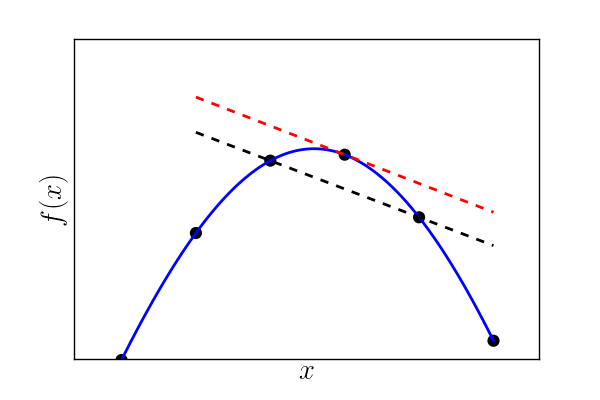
\includegraphics[bb=30bp 10bp 550bp 370bp,clip,width=1\textwidth]{images/fin_dif}
\[
\frac{df}{dx}\approx\frac{\Delta f}{\Delta x}=\frac{f\left(x_{i+1}\right)-f\left(x_{i-1}\right)}{x_{i+1}-x_{i-1}}
\]

\par\end{center}

\end{columns}

\end{frame}

\begin{frame}{Finite Volume Methods}

\begin{columns}[c]


\column{5cm}
\begin{itemize}
\item Break problem domain into a \emph{finite} set of sub-\textbackslash{}emph\{volumes\}.
\item Solve for volume \emph{integral} of quantities inside. Typically
reduces problem into flux calculation across faces of the volume. 
\item If fluxes depend on derivatives then another method (e.g. finite differences)
must be used to find them.
\end{itemize}

\column{5cm}

\[
\frac{d}{dt}\int_{\Omega_{i}}\rho dV=\sum_{\mbox{faces}}\int_{\delta\Omega_{i}^{(j)}}\rho\bm{u}\cdot\bm{n}dS
\]


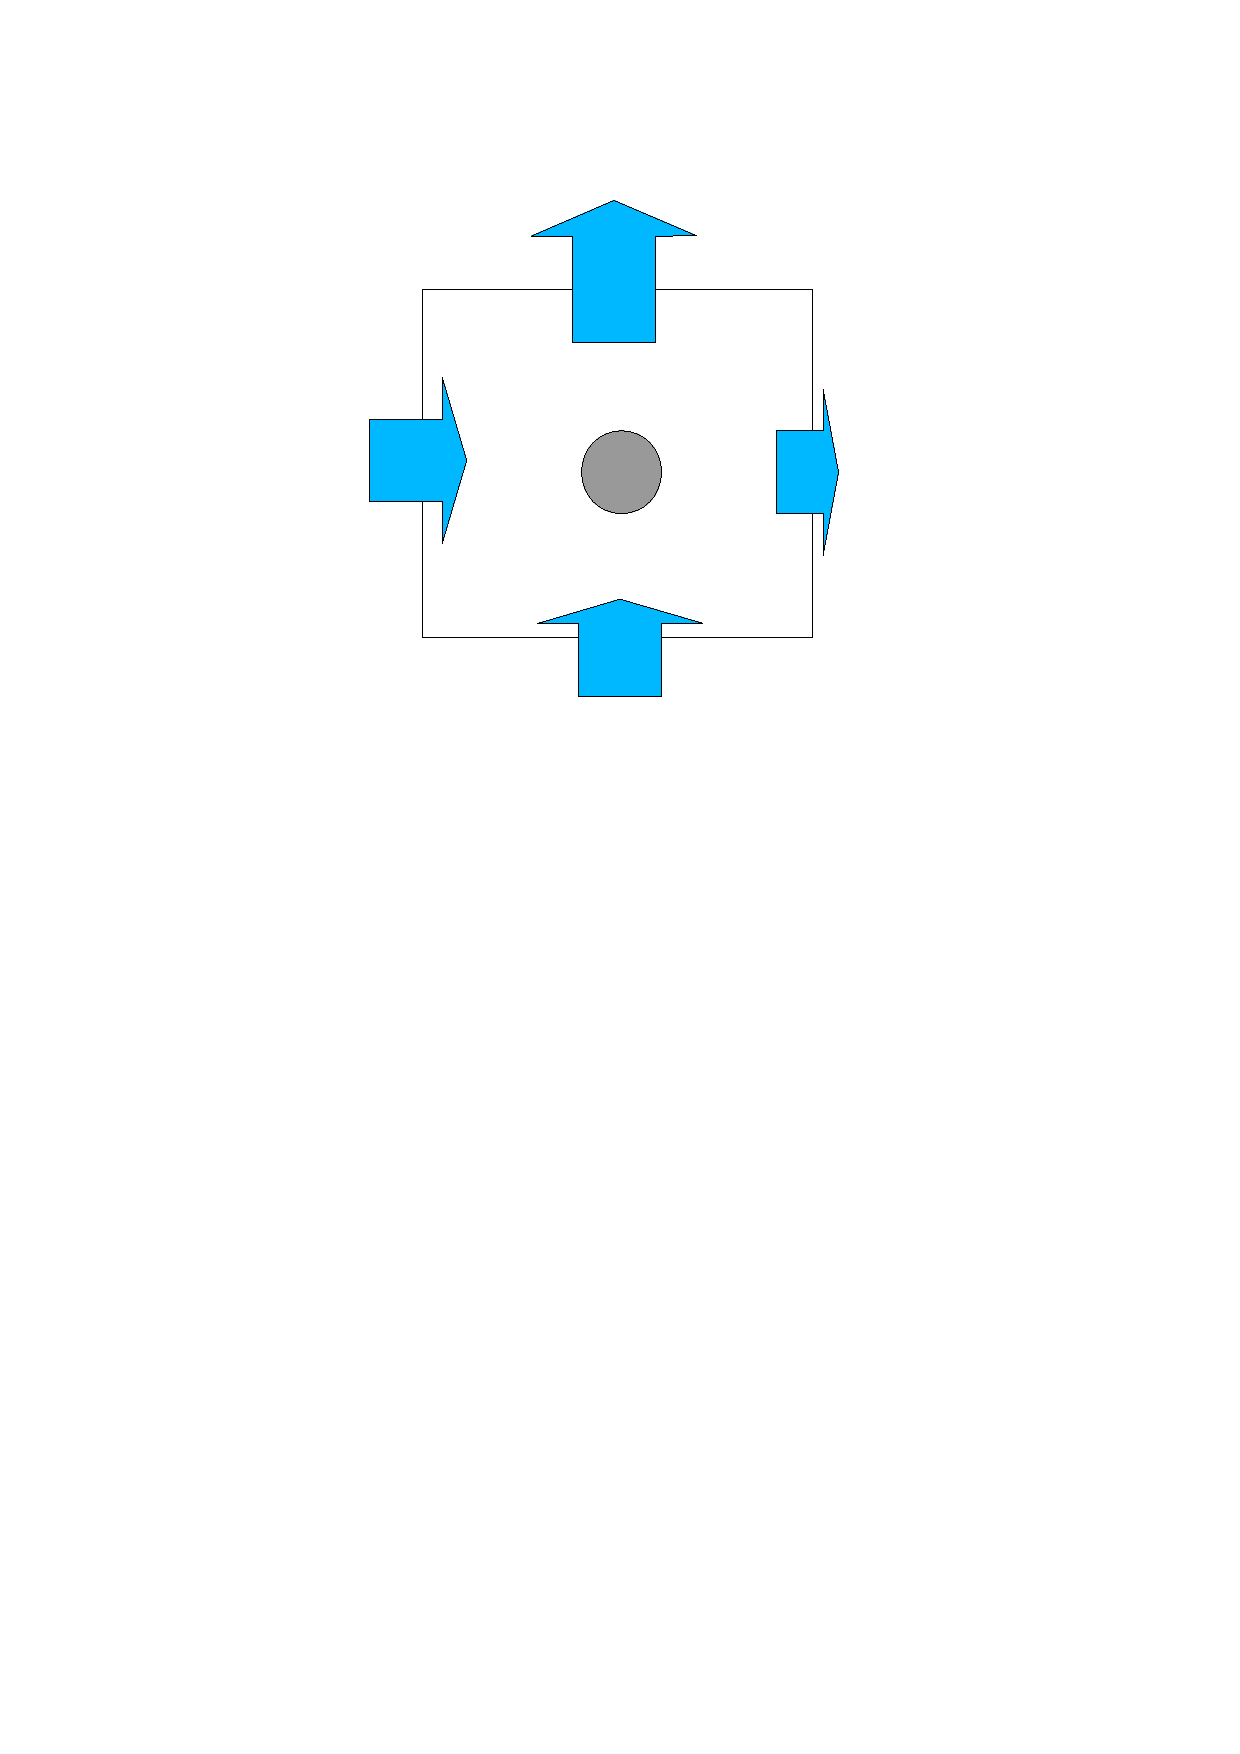
\includegraphics[width=1\textwidth]{images/FVex_crop}


\end{columns}

\end{frame}

\begin{frame}{Spectral Methods}

\begin{columns}[c]


\column{5cm}
\begin{itemize}
\item Represent variables as (limit of) sum of orthogonal \emph{basis functions}.
\item \emph{Global} basis functions vary over entire domain.
\item Truncate infinite series and calculate behaviour of finite set of
coefficients.
\end{itemize}

\column{5cm}


\begin{alignat*}{1}
f\left(x\right) & =\sum_{n=1}^{\infty}a_{n}\cos\left(nx\right)+b_{n}\sin\left(nx\right)\\
 & \approx\sum_{n=1}^{N}a_{n}\cos\left(nx\right)+b_{n}\sin\left(nx\right)
\end{alignat*}



\begin{center}
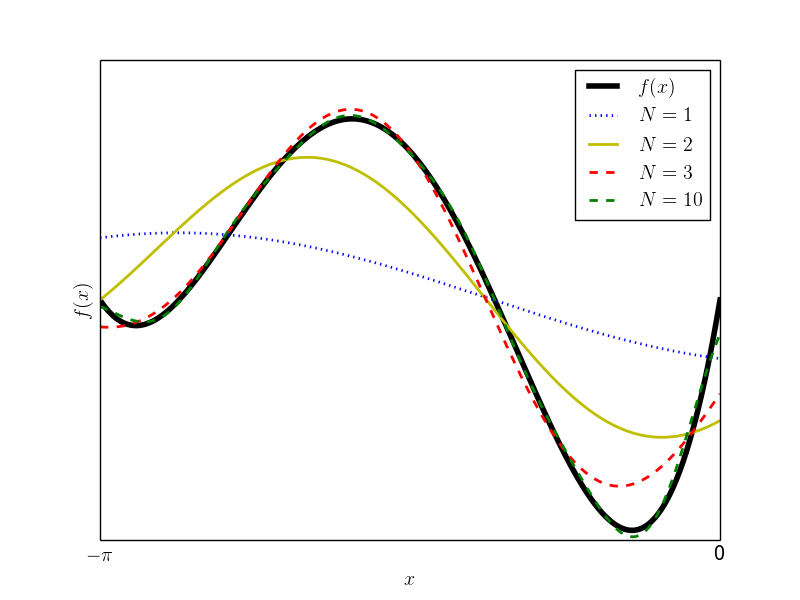
\includegraphics[width=1\textwidth]{images/spec_ex}
\par\end{center}


\end{columns}

\end{frame}

\begin{frame}{Spectral Methods}


\begin{center}
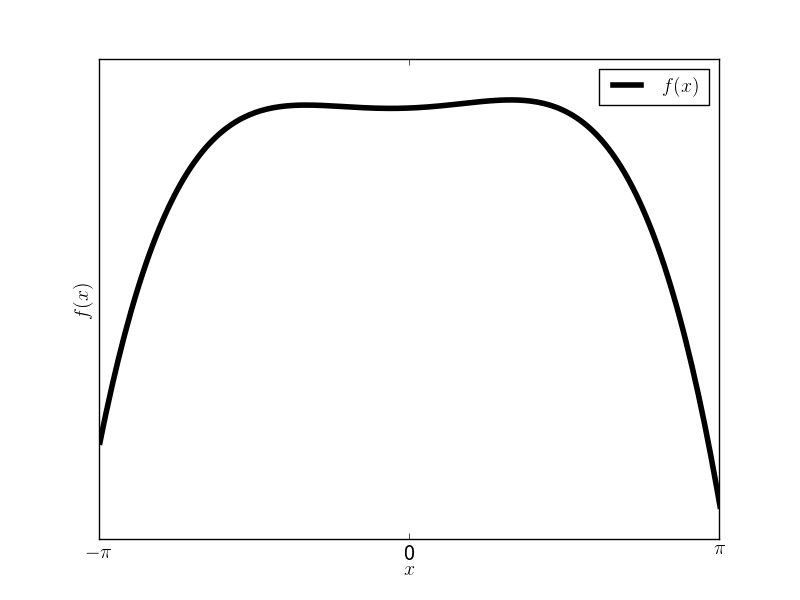
\includegraphics[height=0.9\textheight]{images/spec_ex_0}
\par\end{center}

\end{frame}

\begin{frame}{Spectral Methods}


\begin{center}
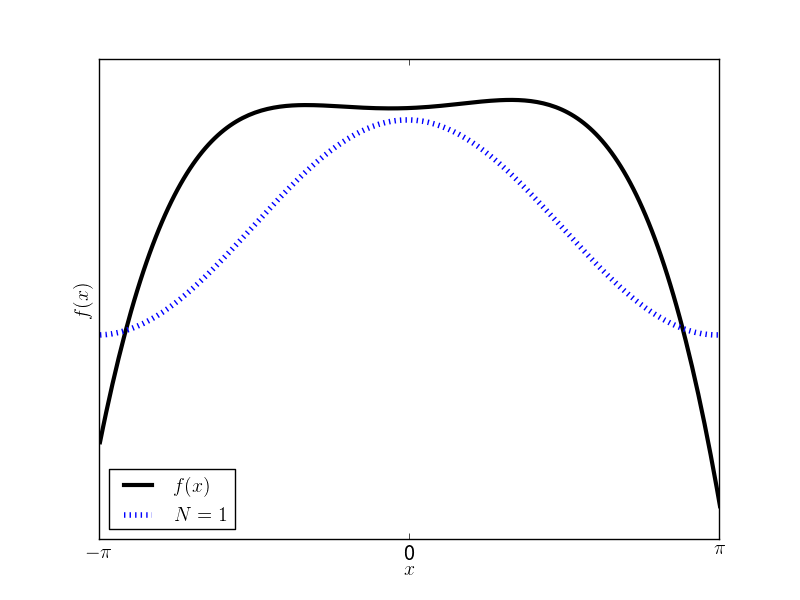
\includegraphics[height=0.9\textheight]{images/spec_ex_1}
\par\end{center}

\end{frame}

\begin{frame}{Spectral Methods}


\begin{center}
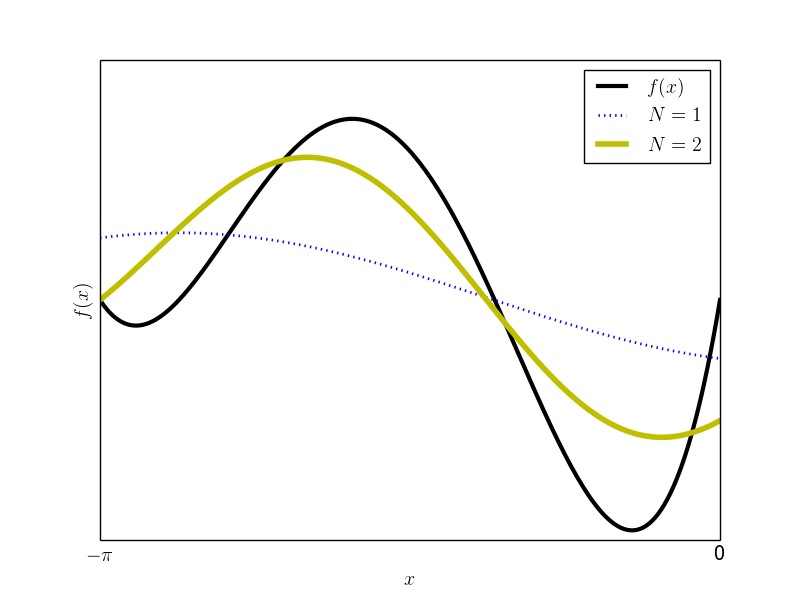
\includegraphics[height=0.9\textheight]{images/spec_ex_2}
\par\end{center}

\end{frame}

\begin{frame}{Spectral Methods}


\begin{center}
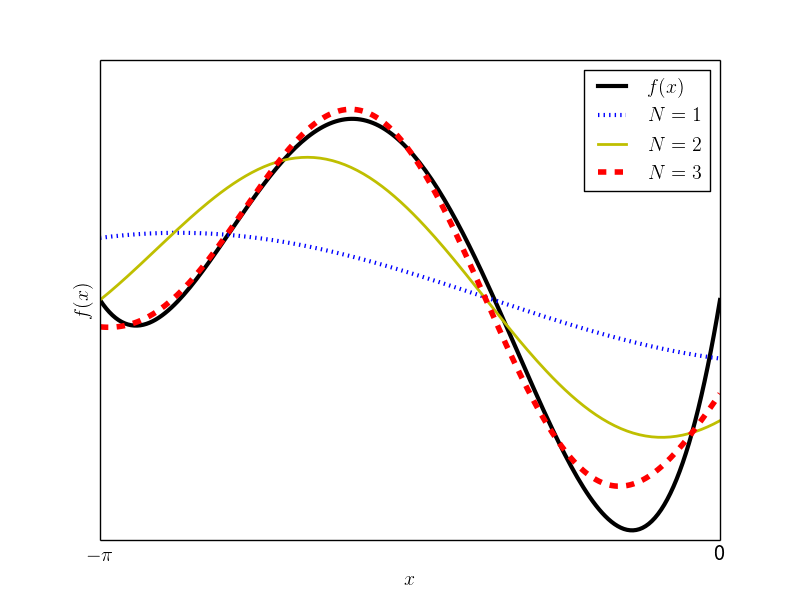
\includegraphics[height=0.9\textheight]{images/spec_ex_3}
\par\end{center}

\end{frame}

\begin{frame}{Finite Element Methods}

\begin{itemize}
\item Break the problem domain down into a finite set of sub-volumes (\emph{elements}). 
\item Represent variables as a sum of \emph{basis functions}.
\item Basis functions non-zero only on \emph{local} set of subvolumes.
\item Solve \emph{integral equation} form of PDE. 
\end{itemize}
\end{frame}

\begin{frame}{Hybrid Methods}

\begin{itemize}
\item Very common to combine these different approaches

\begin{itemize}
\item Couple finite volume method for globally conserved quanity to finite
difference method to calculate fluxes
\item Couple finite volume method for globally conserved quanity to finite
element method to calculate fluxes. ``\emph{Control Volume}'' method
\item Fluidity velocity solver: Finite element method in space, finite difference
in time
\end{itemize}
\end{itemize}



\end{frame}

\section{Finite Elements from First Principles}


\subsection[Prerequisites]{Example: Poisson equation}
\begin{frame}{Poisson Equation: Pressure in Navier-Stokes}


\framesubtitle{Finding pressure in the incompressible Navier-Stokes Equations}
\begin{block}<1->{Incompressible Navier-Stokes equations}


\begin{alignat*}{1}
\tag{momentum}\frac{\partial\bm{u}}{\partial t}+\bm{u}\cdot\nabla\bm{u} & =-\nabla p+\nu\nabla^{2}\bm{u},\\
\tag{continuity}\nabla\cdot\bm{u} & =0,
\end{alignat*}


\end{block}

Taking divergence
\[
\underbrace{\frac{\partial}{\partial t}\left(\nabla\cdot\bm{u}\right)}_{=0}+\nabla\cdot\left(\bm{u}\cdot\nabla\bm{u}\right)=-\nabla^{2}p+\underbrace{\nu\nabla^{2}\nabla\cdot\bm{u}}_{=0}.
\]
I.e.
\[
\nabla^{2}p=-\nabla\cdot\left(\bm{u}\cdot\nabla\bm{u}\right).
\]


\end{frame}

\begin{frame}{ Poisson Equation}


General form of this equation
\begin{block}{Poisson Equation}


\[
\tag{*}\nabla^{2}\psi+f\left(\bm{x}\right)=0,\quad\forall\bm{x}\in\Omega
\]


\end{block}

In 1D, setting $\Omega$ to the unit interval:
\[
\frac{\partial^{2}\psi}{\partial x^{2}}+f\left(x\right)=0\quad\forall x\in(0,1).
\]
This is the \emph{strong form} of the Poisson equation.

\end{frame}

\subsection{Strong and Weak Forms}
\begin{frame}{Strong Form vs. Weak Form of an Equation}

\begin{columns}[t]


\column{5cm}
\begin{block}{Strong form}


Equation ({*}) true individually for each point in space,

\[
\nabla^{2}\psi+f\left(x\right)=0,
\]
for all $x$ in domain $\Omega$.

Test a $\psi$ by checking equation holds individually for each point
in space.
\end{block}

\column{6cm}
\begin{block}{Weak form}


Integral equation holds for all choices of a `\emph{test function}',
$\phi$,
\[
\int_{\Omega}\phi\left(\nabla^{2}\psi+f\right)\, dV=0,
\]
where $\phi:\Omega\rightarrow\mathbb{R}$ is from a function space
defined later.

Test possible $\psi$ (`\emph{trial function}') by checking integral
equation holds for all \emph{test functions}, $\phi$.
\end{block}
\end{columns}

\end{frame}

\begin{frame}{Quick Review of Vector Spaces}


A set, $\mathcal{V}$, is a vector space if it has + (addition) and
scalar multiplication operators where 
\begin{alignat*}{1}
\tag{associativity}\bm{a}+\left(\bm{b+\bm{c}}\right) & =\left(\bm{a}+\bm{b}\right)+\bm{c},\\
\tag{commutivity}\bm{a}+\bm{b} & =\bm{b}+\bm{a},\\
\mbox{there exists }\bm{0}\in\mathcal{V}\mbox{ such that } & \bm{a}+\bm{0}=\bm{a},\mbox{ for all }\bm{a}\in\mathcal{V},\\
\mbox{for all }\bm{a}\mbox{ there exists }-\bm{a}\in\mathcal{V} & \mbox{ such that }\bm{a}+\left(-\bm{a}\right)=\bm{0},\\
\tag{distributivity I}\alpha\left(\bm{a}+\bm{b}\right) & =\alpha\bm{a}+\alpha\bm{b},\\
\tag{distributivity II}\left(\alpha+\beta\right)\bm{a} & =\alpha\bm{a}+\beta\bm{a},\\
\alpha\left(\beta\bm{a}\right) & =\left(\alpha\beta\right)\bm{a},\\
1\bm{a} & =\bm{a}.
\end{alignat*}


\end{frame}

\begin{frame}{Vector Spaces}


Functions are a vector space under the following definitions of addition
and scalar multiplication:


\begin{alignat*}{1}
\left(f+g\right)\left(x\right) & =f\left(x\right)+g\left(x\right),\\
\left(\alpha f\right)\left(x\right) & =\alpha\left(f\left(x\right)\right).
\end{alignat*}



I.e. functions are added/multiplied pointwise based on their result.
Necessary axioms all follow from the normal rules of addition/multiplication.

\end{frame}

\begin{frame}{Vector Spaces}


\begin{center}
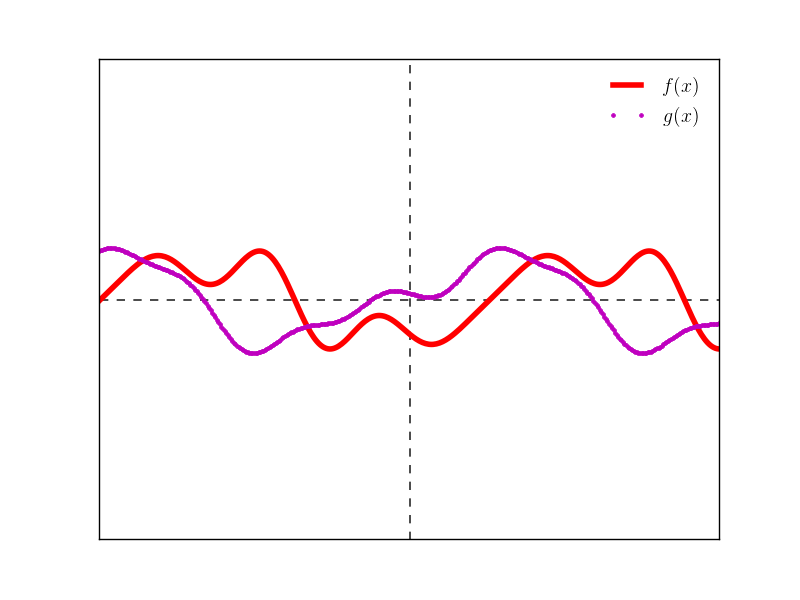
\includegraphics[width=0.8\textwidth]{images/add_fns_0}
\par\end{center}

\end{frame}

\begin{frame}{Vector Spaces}


\begin{center}
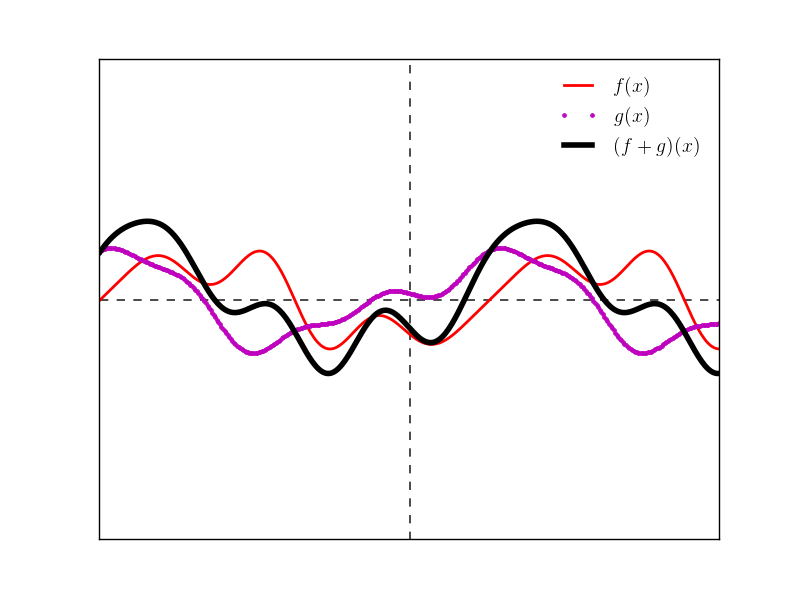
\includegraphics[width=0.8\textwidth]{images/add_fns_1}
\par\end{center}

\end{frame}

\begin{frame}{Vector Spaces}


\begin{center}
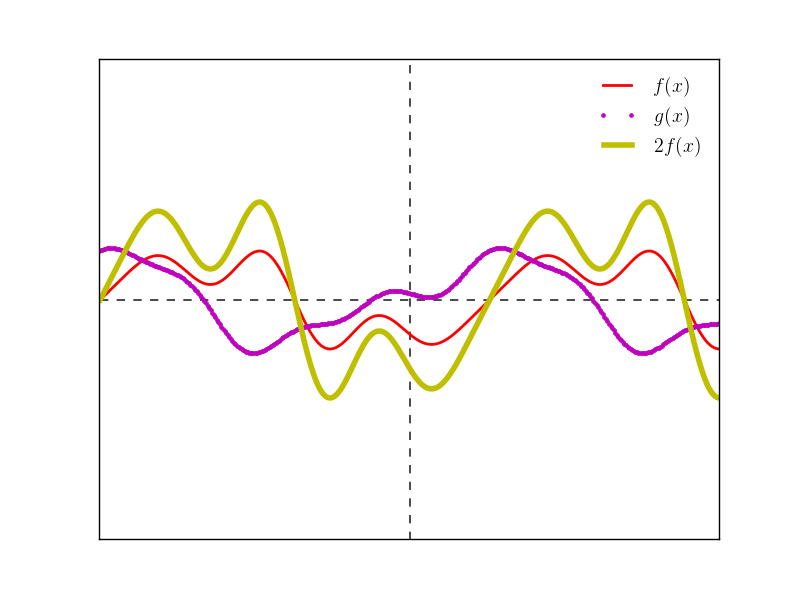
\includegraphics[width=0.8\textwidth]{images/add_fns_2}
\par\end{center}

\end{frame}

\begin{frame}{Vector Spaces}


Within the space of functions there are many smaller subspaces. Eg:
\begin{exampleblock}{Examples}


Polynomials $f(x)=1+3x+4x^{2}+5x^{3}$

Functions on an interval $f(x)=\begin{cases}
0 & x<0,\\
e^{x} & 0\leq x\leq1,\\
0 & x>1.
\end{cases}$

Twice differentiable functions $f\left(x\right)=\begin{cases}
x^{2}+2, & x<0,\\
2\left(e^{x}-x\right). & x\geq0.
\end{cases}$
\end{exampleblock}
\end{frame}

\begin{frame}{Vector Spaces}


Key idea of finite element method: 
\begin{itemize}
\item Desire an exact solution $\psi$, from an inifinite dimensional vector
space, $\mathcal{V}$, which satisfies weak form equation, for test
functions $\phi$ in $\mathcal{U}$.
\item Find $\psi^{\delta}$ in approximate vector (sub)space $\mathcal{V}^{\delta}\subset\mathcal{V}$
with finite representation, which satisfies same weak form equation,
for test functions $\phi^{\delta}$ in approximate space $\mathcal{U}^{\delta}\subset\mathcal{U}$.
\item Expectation that as $\delta\rightarrow0$, $\mathcal{V}^{\delta}\rightarrow\mathcal{V}$
and $\psi^{\delta}\rightarrow\psi$.
\end{itemize}
\end{frame}

\begin{frame}{Strong and Weak Forms}


A solution to the strong form of the equations \emph{will} be a solution
to the weak form equations:


If $\nabla^{2}\psi+f=0$ then
\[
\int\phi\left(\nabla^{2}\psi+f\right)\: dV=\int\phi\cdot0\: dV=0,
\]



independent of $\phi$, i.e. for any possible choice of test space.

\end{frame}

\begin{frame}{Strong and Weak Forms}


A solution to the weak form of the equations \emph{may} be a solution
to the strong equations if it is smooth enough.


The weak formulation extends the equations to allow non-smooth solutions
which exist in a distributional sense.
\begin{exampleblock}{Examples of common distributions}


\[
\tag{Dirac delta}\delta\left(x\right),\quad\int_{-\infty}^{a}f\left(x\right)\delta\left(x\right)=\begin{cases}
f\left(0\right), & a>0,\\
0, & a<0.
\end{cases}
\]
\[
\tag{Heaviside}H\left(x\right):=\int_{-\infty}^{x}\delta\left(s\right)ds=\begin{cases}
0, & x<0,\\
1, & x>0.
\end{cases}
\]


\end{exampleblock}
\end{frame}

\begin{frame}{Example of a Weak Nonclassical Solution}


\[
\tag{Helmholtz}\psi-\nabla^{2}\psi\left(x\right)=a\delta\left(X-x\right)
\]
\[
\psi=\begin{cases}
a\text{\ensuremath{\exp\left(x-X\right)}} & x\leq X,\\
a\exp\left(X-x\right) & x>X
\end{cases}
\]



\begin{center}
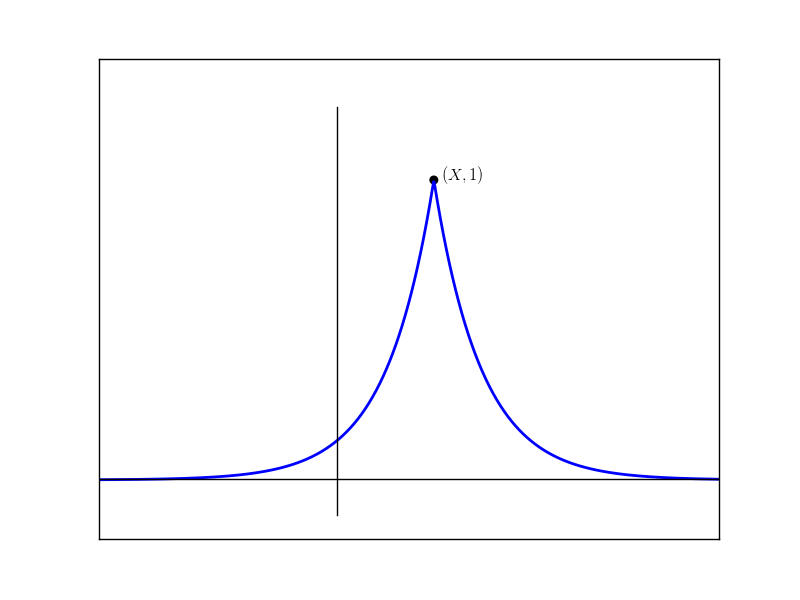
\includegraphics[width=0.6\textwidth]{peakon}
\par\end{center}

\end{frame}

\begin{frame}{Review of Section}

\begin{itemize}
\item \emph{Strong} form of PDEs prescribes behaviour \emph{pointwise}

\begin{itemize}
\item Finite difference methods work at a finite number of points
\end{itemize}
\item \emph{Weak} form of PDEs prescribes behaviour over intervals (areas,
volumes etc.)

\begin{itemize}
\item Finite element methods work over a finite number of intervals
\end{itemize}
\item Functions live in vector spaces, which can be approximated.
\end{itemize}
\end{frame}

\subsection{Boundary Conditions}
\begin{frame}{Boundary Conditions for Weak Equations}


Two possible forms of boundary condition for a solution to the Poisson
equation to be well posed:
\begin{enumerate}
\item Dirichlet: $\psi(x)=a(x)$ for $x\in A\subset\delta\Omega$,
\item Neumann: $\frac{\partial\psi}{\partial x}=b\left(x\right)$ for $x\in B\subset\delta\Omega$.
\end{enumerate}

In the Galerkin formulation, \emph{Dirichlet} boundary conditions
typically require explicit \emph{modification} of the structure of
the problem to be solved, whereas \emph{Neumann} conditions are dealt
with \emph{naturally} as part of the formulation. We'll use a Dirichlet
boundary condition at $x=0$, and a Neumann condition at $x=1$ in
our example.

\end{frame}

\begin{frame}{Natural Boundary Conditions}


Our weak form equation is


\[
\int_{0}^{1}\phi\left(\frac{\partial^{2}\psi}{\partial x^{2}}+f\right)\: dx=0,
\]
Integrate by parts,
\[
\int_{0}^{1}\frac{\partial\phi}{\partial x}\frac{\partial\psi}{\partial x}\, dx-\int_{0}^{1}\phi f\, dx=-\left[\phi\frac{\partial\psi}{\partial x}\right]_{0}^{1}.
\]
Chose $\phi$ to vanish on Dirichlet boundaries (and set $\psi=a(0)$),
and use our knowlege of $\frac{\partial\psi}{\partial x}$ on Neumann
boundaries:
\[
\int_{0}^{1}\frac{\partial\phi}{\partial x}\frac{\partial\psi}{\partial x}\, dx=\int_{0}^{1}\phi f\, dx-\phi\left(1\right)b\left(1\right)
\]


\end{frame}

\begin{frame}{Dirichlet Boundary Conditions}


Dirichlet boundary conditions can be enforced through splitting solution
into two parts


\[
\psi=\psi_{0}+\psi_{d}
\]
where $\psi_{d}$ is any (chosen) function satisfying 
\[
\psi_{d}\left(0\right)=a(0),\qquad\frac{\partial\psi_{d}}{\partial x}\left(1\right)=0
\]
while $\psi_{0}$ satisfies a modified weak equation, with $\psi_{d}$
on r.h.s,
\[
\psi_{0}(0)=0,
\]
\[
\int_{0}^{1}\frac{\partial\phi}{\partial x}\frac{\partial\psi_{0}}{\partial x}\: dx=\int_{0}^{1}\phi f\: dx-\phi\left(1\right)b\left(1\right)-\int_{0}^{1}\frac{\partial\phi}{\partial x}\frac{\partial\psi_{d}}{\partial x}\: dx,
\]



Note $\psi_{0}$ vanishes on the Dirichlet boundaries, same condition
we apply to $\phi$.

\end{frame}

\begin{frame}{Boundary Conditions: Strong vs. Weak}


More generally, implementations of finite element boundary conditions
come in two flavours, strong and weak.
\begin{columns}


\column{5cm}
\begin{block}{Strong form bc.s}


Information contained in boundary condition appears implicitly in
the weak form of the PDE. Solve by lifting method.
\end{block}

\column{5cm}
\begin{block}{Weak form bcs.}


Information contained in boundary condition appears explicitly in
surface integrals in the weak form of the PDE. Solve by direct substitution.
\end{block}
\end{columns}

\end{frame}

\begin{frame}{Boundary Conditions: Strong vs. Weak}


Which method to apply depends on the details of both the original
PDE and the weak form to be solved. Sometimes both are possible. 


For example, consider solving the advection equation,
\[
\frac{\partial\tau}{\partial t}+\bm{a}\cdot\nabla\tau=0,
\]
for a tracer $\tau$, given a known velocity field, $\bm{a}$ and
dirichlet boundary conditions at a inlet.


Note the odd number of spatial derivatives, whereas even number for
Poisson equation.

\end{frame}

\begin{frame}{Boundary Conditions: Strong vs. Weak}

\begin{columns}


\column{5cm}
\begin{block}{Strong form bc.s}


Solve 
\[
\int_{\Omega}\phi\left(\frac{\partial\tau}{\partial t}+\bm{a}\cdot\nabla\tau\right)dx=0,
\]


Dirichlet bcs must be applied strongly.
\end{block}

\column{5cm}
\begin{block}{Weak form bcs.}


Integrate by parts,
\begin{alignat*}{1}
\int_{\Omega}\phi\frac{\partial\tau}{\partial t}-\tau\nabla\cdot\left(\phi\bm{a}\right)dx\\
\qquad=-\int_{\delta\Omega^{+}}\bm{a}\cdot\bm{n}\phi\tau_{b}\: dS,
\end{alignat*}


where $\tau_{b}$ is the Dirichlet bc, applied weakly.
\end{block}
\end{columns}


When using this sort of weak boundary condition, values may not be
quite what you'd expect, however fluxes should be right.

\end{frame}

\begin{frame}{Finite Element Basis Functions}


Need discrete finite dimensional representation of problem to do numerical
calculations on a computer. Set
\[
\psi^{\delta}\left(x\right)=\sum_{i=1}^{N}\hat{\psi}_{i}N_{i}\left(x\right)
\]
where $\hat{\psi}_{i}\in\mathbb{R}$ is a scalar parameter and $N_{i}:\Omega\rightarrow\mathbb{R}$
is a fixed shape function specifing spatial dependence. Can do the
same for the space of test functions, $\phi$.

\end{frame}

\begin{frame}{Finite Element Functions}


For our 1D Poisson equation example we can choose to use the set of
continuous, piecewise linear functions ('\emph{shape functions}')
on subdivisions of the unit interval.
\[
N_{i}=\begin{cases}
0, & x\leq x_{(i-1)},\\
\frac{x-x_{(i-1)}}{x_{i}-x_{(i-1)}}, & x_{(i-1)}<x\leq x_{i},\\
\frac{x_{(i+1)}-x}{x_{(i+1)}-x_{i}}, & x_{i}<x\leq x_{(i+1)},\\
0. & x>x_{(i+1)}.
\end{cases}
\]
Functions are equal to 1 at the set of points $[0,x_{1,}x_{2},\ldots x_{n-1},1]$,
sometimes called 'nodes' or 'degrees of freedom'. The subdivisions
of $\Omega$ over which the $N_{i}$s are smooth are often called
\emph{elements}.

\end{frame}

\begin{frame}{Finite Element Functions}


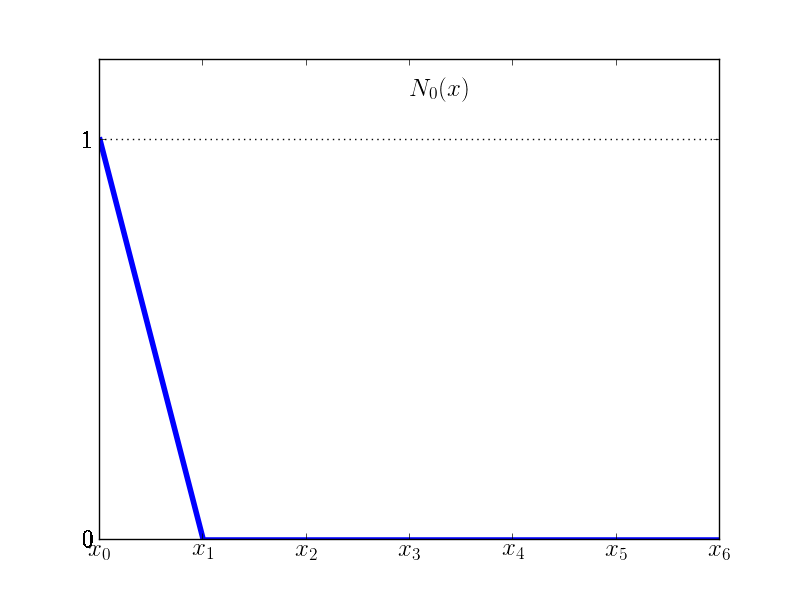
\includegraphics[width=1\textwidth]{images/N_0}

\end{frame}

\begin{frame}{Finite Element Functions}


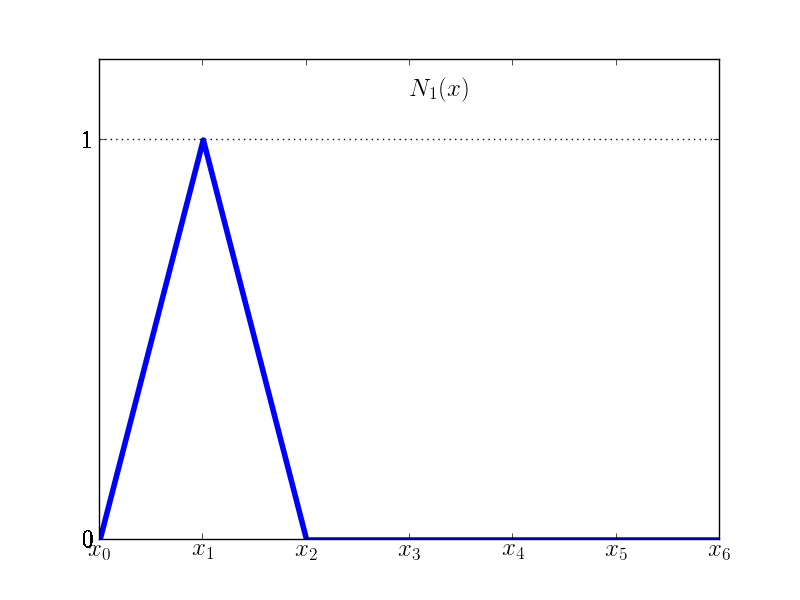
\includegraphics[width=1\textwidth]{images/N_1}

\end{frame}

\begin{frame}{Finite Element Functions}


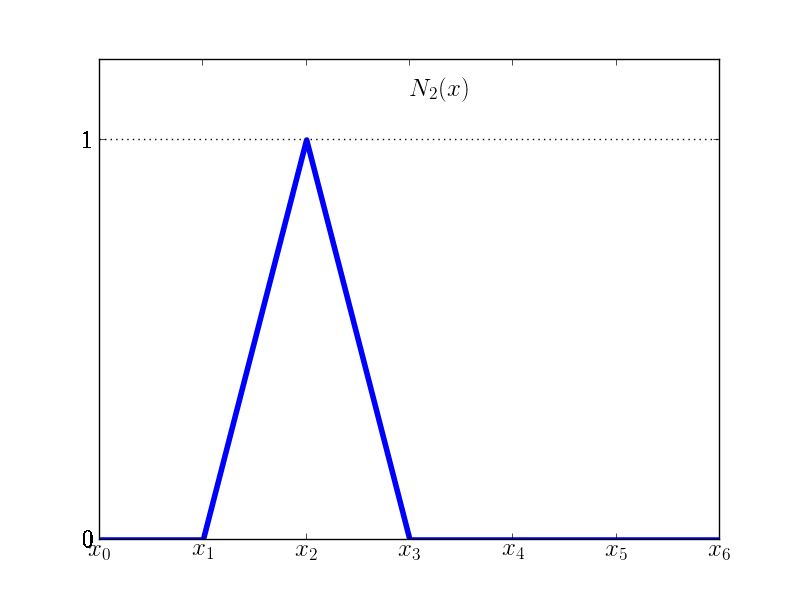
\includegraphics[width=1\textwidth]{images/N_2}

\end{frame}

\begin{frame}{Finite Element Functions}


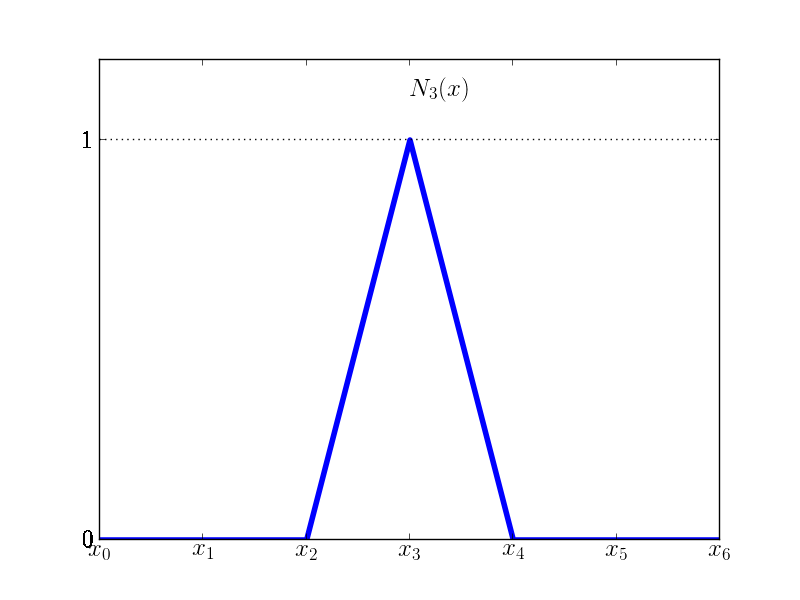
\includegraphics[width=1\textwidth]{images/N_3}

\end{frame}

\begin{frame}{Finite Element Functions}


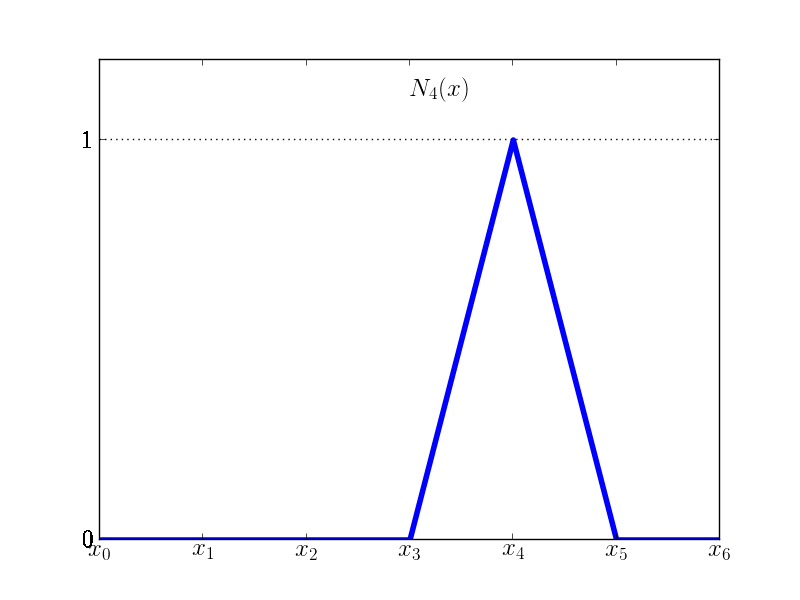
\includegraphics[width=1\textwidth]{images/N_4}

\end{frame}

\begin{frame}{Finite Element Functions}


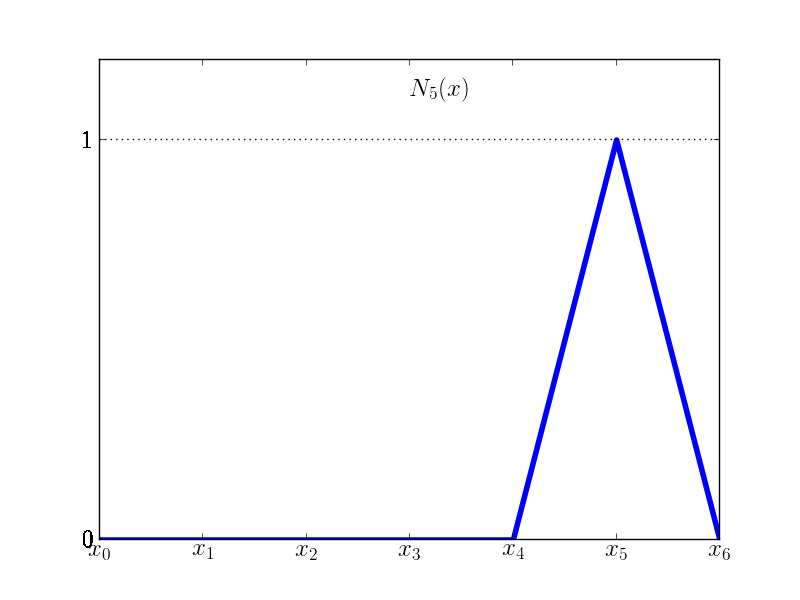
\includegraphics[width=1\textwidth]{images/N_5}

\end{frame}

\begin{frame}{Finite Element Functions}


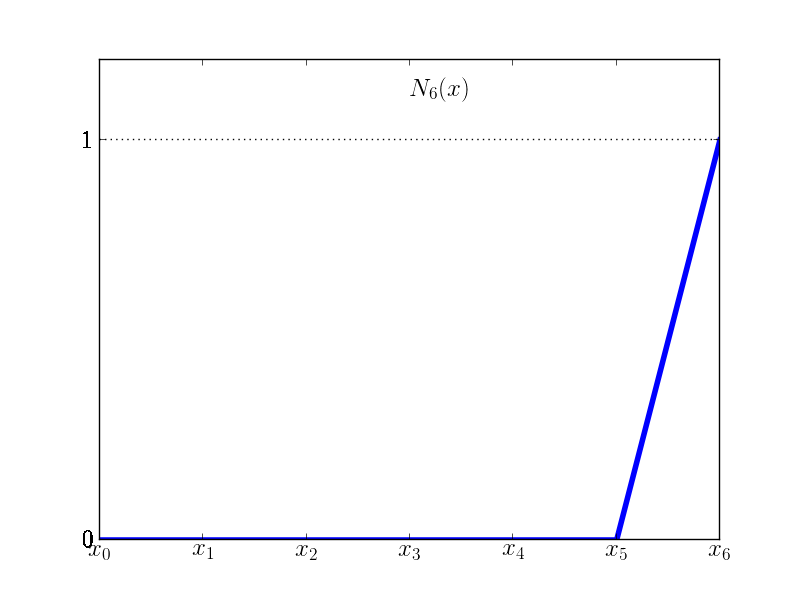
\includegraphics[width=1\textwidth]{images/N_6}

\end{frame}

\begin{frame}{Galerkin Approximation}


To obtain the Galerkin approximation of the Poisson equation, we find
the (unique) solution of the weak form equation when $\psi$ and $\phi$
are approximated by our finite element expansions, 
\begin{alignat*}{1}
\psi^{\delta} & =\sum_{i=0}^{n}\hat{\psi}_{i}N_{i},\\
\phi^{\delta} & =\sum_{j=0}^{n}\hat{\phi}_{j}N_{j}.
\end{alignat*}



The $\psi^{\delta}$ are called \emph{trial functions} and the function
space they come from is the trial space. The $\phi^{\delta}$are called
\emph{test functions} and live in the trial space. Computation involves
obtaining the \emph{finite} number of $\hat{\psi}_{i}$. Can then
be solved on a computer.

\end{frame}

\begin{frame}{Galerkin Approximation}


Substituing the finite representations into ({*}) we get


\begin{alignat*}{1}
\int\sum_{j=1}^{n}\hat{\phi}_{j}\frac{\partial N_{j}}{\partial x}\sum_{i=1}^{N}\hat{\psi}_{i}\frac{\partial N_{i}}{\partial x}\: dV+v_{N}^{\delta}b\left(x_{N}\right) & =\int\sum_{j=1}^{n}\hat{\phi}_{j}^{\delta}N_{j}f\: dV,
\end{alignat*}



\begin{alignat*}{1}
\hat{\phi}_{j}\left(\underbrace{\left[\int\frac{\partial N_{j}}{\partial x}\frac{\partial N_{i}}{\partial x}dV\right]}_{\mathrm{matrix\,}D_{ij}}\hat{\psi}_{i}-\int fN_{j}dV+\begin{cases}
0, & j=1,\ldots n-1\\
b\left(x_{n}\right), & j=n
\end{cases}\right)\\
=0\qquad\qquad
\end{alignat*}
If bracket vanishes, solution applies for any $\hat{\phi}_{j}$, so
we can drop them. 

\end{frame}

\begin{frame}{The Right Hand Side}


Generally the right hand side of the equation is known explicitly
as a function $f:\Omega\rightarrow\mathbb{R}$. Hence $\int_{0}^{1}\phi^{\delta}f\, dx$
can be calculated exactly. In practice (especially for coupled problems,)
it is usually represented in the approximate function space,
\[
f^{\delta}\left(x\right)=\sum_{i=1}^{N}\hat{f}_{i}N_{i}\left(x\right),
\]
where, for our choice of shape functions,
\[
\hat{f}_{i}=f\left(x_{i}\right).
\]


\end{frame}

\begin{frame}{Finite Element Poisson Matrix Problem}


Dirichlet condition: $\hat{\psi}_{0}=a(0)$, turns up on right hand
side:


\begin{center}
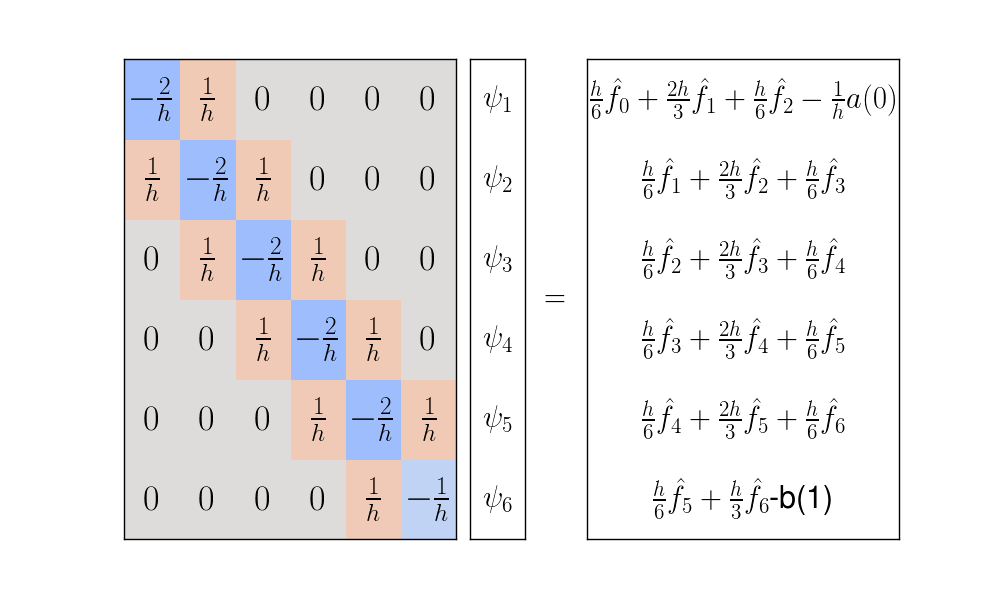
\includegraphics[width=0.9\textwidth]{images/FEmatrix}
\par\end{center}

\end{frame}

\begin{frame}{Local to global}


Note that
\begin{alignat*}{1}
D_{ij} & =\int_{\Omega}\frac{\partial N_{i}}{\partial x}\frac{\partial N_{j}}{\partial x}\: dV,\\
 & =\sum_{k}\int_{\Omega^{(k)}}\frac{\partial N_{i}}{\partial x}\frac{\partial N_{j}}{\partial x}\: dV,
\end{alignat*}
where the $\Omega^{k}=[x_{i},x_{i+1}]$ only contribute if
\[
\frac{\partial N_{i}}{\partial x}\neq0,\quad\frac{\partial N_{j}}{\partial x}\neq0.
\]
Global matrix assembled from sum of local integrals over elements.

\end{frame}

\begin{frame}{Finite Difference Poisson Matrix Problem}


Finite Difference discretization of same problem:


\begin{center}
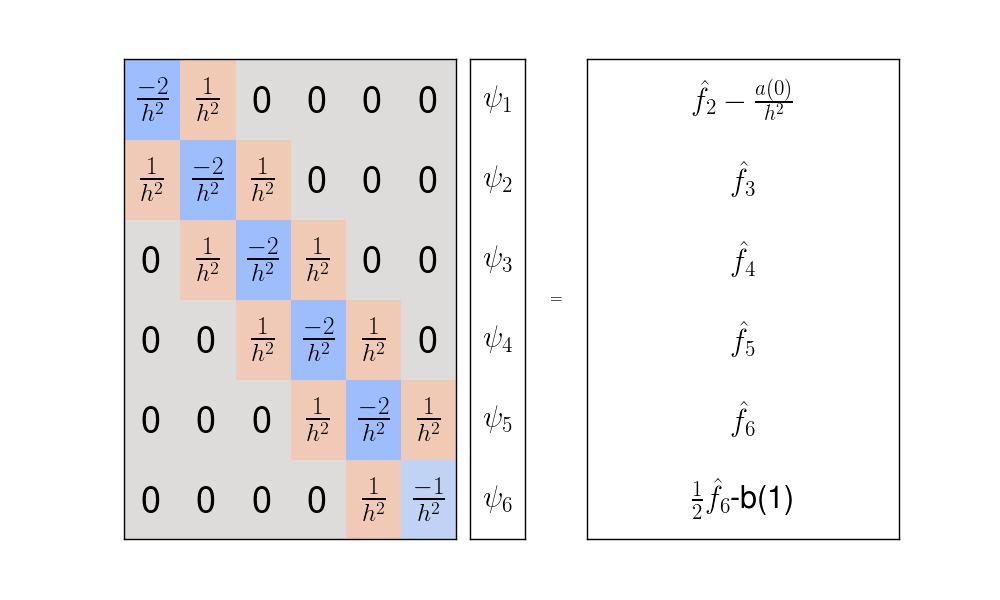
\includegraphics[width=0.9\textwidth]{images/FDmatrix}
\par\end{center}

\end{frame}

\begin{frame}{Finite Volume Poisson Matrix Problem}


Finite volume discretization of same problem. 2 point finite difference
approximation for flux terms:


\begin{center}
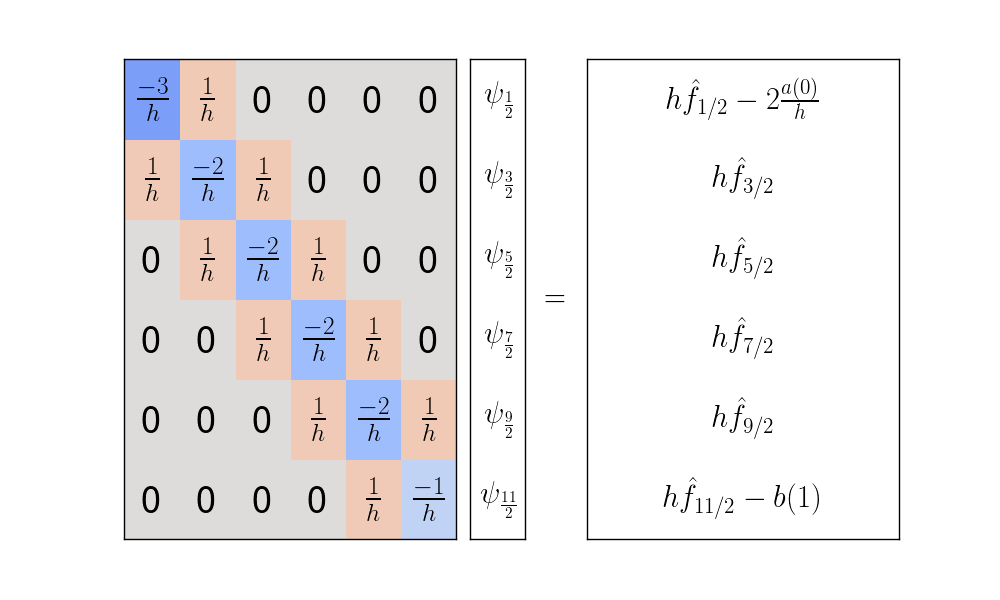
\includegraphics[width=0.85\textwidth]{images/FVmatrix}
\par\end{center}

\end{frame}

\begin{frame}{Solutions: Finite Element}


$f=10\sin\left(5x\right)+\nicefrac{1}{2}\cos\left(3\left(x+\nicefrac{1}{2}\right)\right),$
$\psi\left(0\right)=0$, \textrm{$\frac{d\psi}{dx}=1:$}


\begin{center}
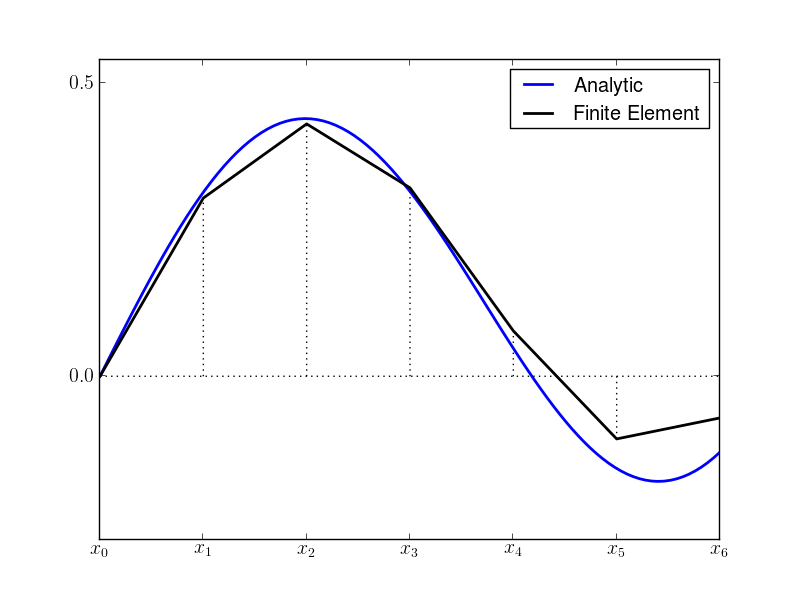
\includegraphics[width=0.9\textwidth]{images/solnFE}
\par\end{center}

\end{frame}

\begin{frame}{Solutions: Finite Difference}


$f=10\sin\left(5x\right)+\nicefrac{1}{2}\cos\left(3\left(x+\nicefrac{1}{2}\right)\right),$
$\psi\left(0\right)=0$, \textrm{$\frac{d\psi}{dx}=1:$}


\begin{center}
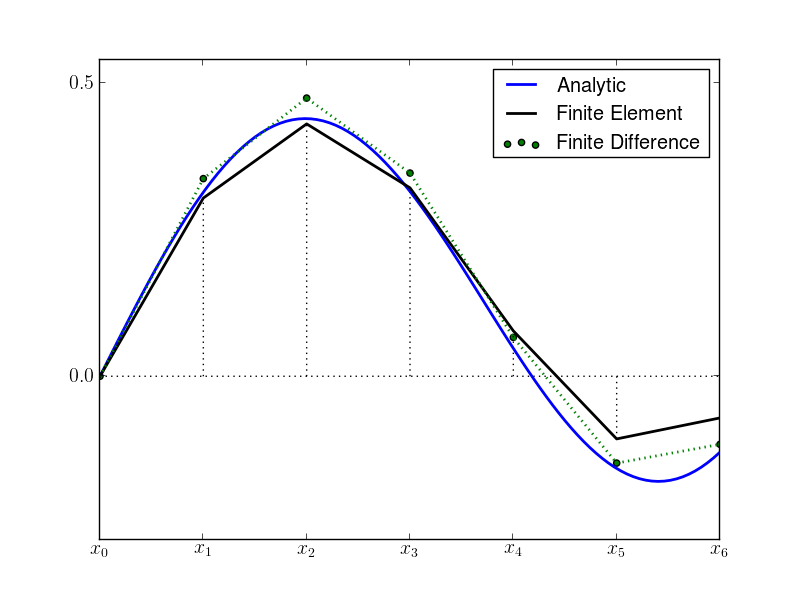
\includegraphics[width=0.9\textwidth]{images/solnFD}
\par\end{center}

\end{frame}

\begin{frame}{Solutions: Finite Volume}


$f=10\sin\left(5x\right)+\nicefrac{1}{2}\cos\left(3\left(x+\nicefrac{1}{2}\right)\right),$
$\psi\left(0\right)=0$, \textrm{$\frac{d\psi}{dx}=1:$}


\begin{center}
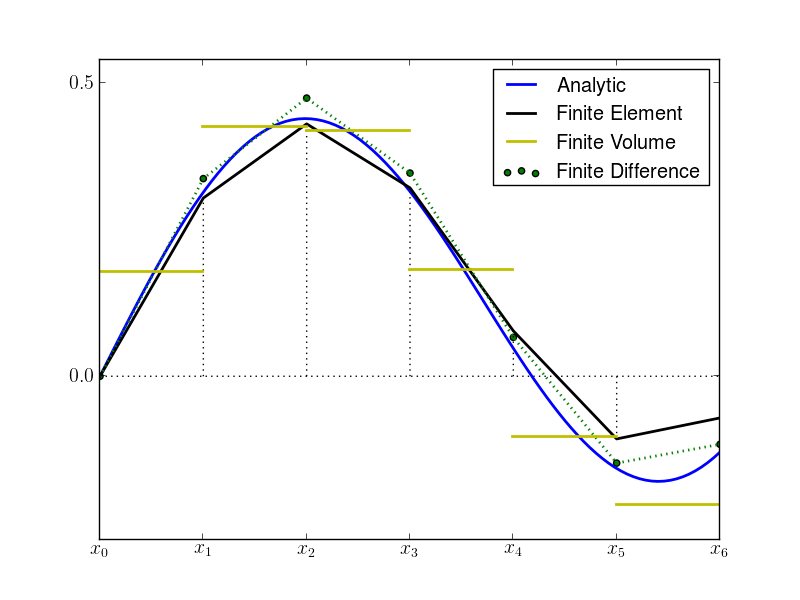
\includegraphics[width=0.9\textwidth]{images/solnFV}
\par\end{center}

\end{frame}

\begin{frame}{Example II: Advection-Diffusion}


Use same finite element framework for 1D advection diffusion equation:


\[
\frac{\partial\tau}{\partial t}+\frac{\partial}{\partial x}\left(u\tau\right)=\frac{\partial}{\partial x}\left(\kappa\frac{\partial\tau}{\partial x}\right)
\]



\[
\int_{0}^{1}\phi\frac{\partial\tau}{\partial t}\, dx=\int\frac{\partial\phi}{\partial x}\left(u\tau-\kappa\frac{\partial\tau}{\partial x}\right)\: dx
\]


\end{frame}

\begin{frame}{Example II: Advection-Diffusion}


Given FEM framework, crank the handle to reduce the problem; Discretize
through Finite Element Galerkin Method,


\[
\tau^{\delta}=\sum_{i=0}^{n}\hat{\tau}_{i}N_{i}^{\tau},
\]
\[
u^{\delta}=\sum_{i=0}^{n}\hat{u}_{i}N_{i}^{u}
\]
\[
\phi^{\delta}=\sum_{i=0}^{n}\hat{\phi}_{i}N_{i}^{\tau},
\]



Note that the method doesn't require $N_{i}^{u}=N_{i}^{\tau}$. \emph{Mixed formulations}
are possible

\end{frame}

\begin{frame}{Example II: Advection-Diffusion}


Following substitution, integrate by parts to obtain


\[
\underbrace{\int_{0}^{1}N_{i}N_{j}\: dx}_{\mbox{"Mass matrix"}M_{ij}}\frac{\partial\hat{\tau}_{j}}{\partial t}-\int_{0}^{1}\frac{\partial N_{i}}{\partial x}\left(N_{j}\sum_{k=0}^{n}u_{k}N_{k}^{u}-\kappa\frac{\partial N_{j}}{\partial x}\right)\: dx\hat{\tau}_{j}=0,
\]



or in matrix form,
\[
\mathrm{M}\frac{\partial\bm{\tau}}{\partial t}+\mathrm{A}\left(\bm{u}\right)\bm{\bm{\tau}}+\mathrm{D}\left(\kappa\right)\bm{\tau}=0,
\]



This is the FEM form of the tracer advection-diffusion equation. Further
details will depend on the choice of shape functions and timestepping
method.

\end{frame}

\begin{frame}{Review of Section}

\begin{itemize}
\item \emph{Finite element} methods solve \emph{weak (integral)} equations
\item Functions get approximated by finite dimensional summations of functions,
non-zero over small regions of problem domain (elements)
\item Linear PDE problem gives a linear (matrix) problem for the $\hat{\psi}_{i}$. 
\end{itemize}

The efficient computational representation and solution of these sorts
of problems will form the basis of the other session.

\end{frame}

\section{Extending the method}


\subsection{Two and Three dimensional FEM}
\begin{frame}{Extensions: Higher dimensions}


The linear finite element method extends naturally on simplicies {[}line
elements, triangle elements, tetrahedrons{]}. Basis functions are
set to 1 at one vertex and to zero on the others. E.g. for triangles:


\begin{center}
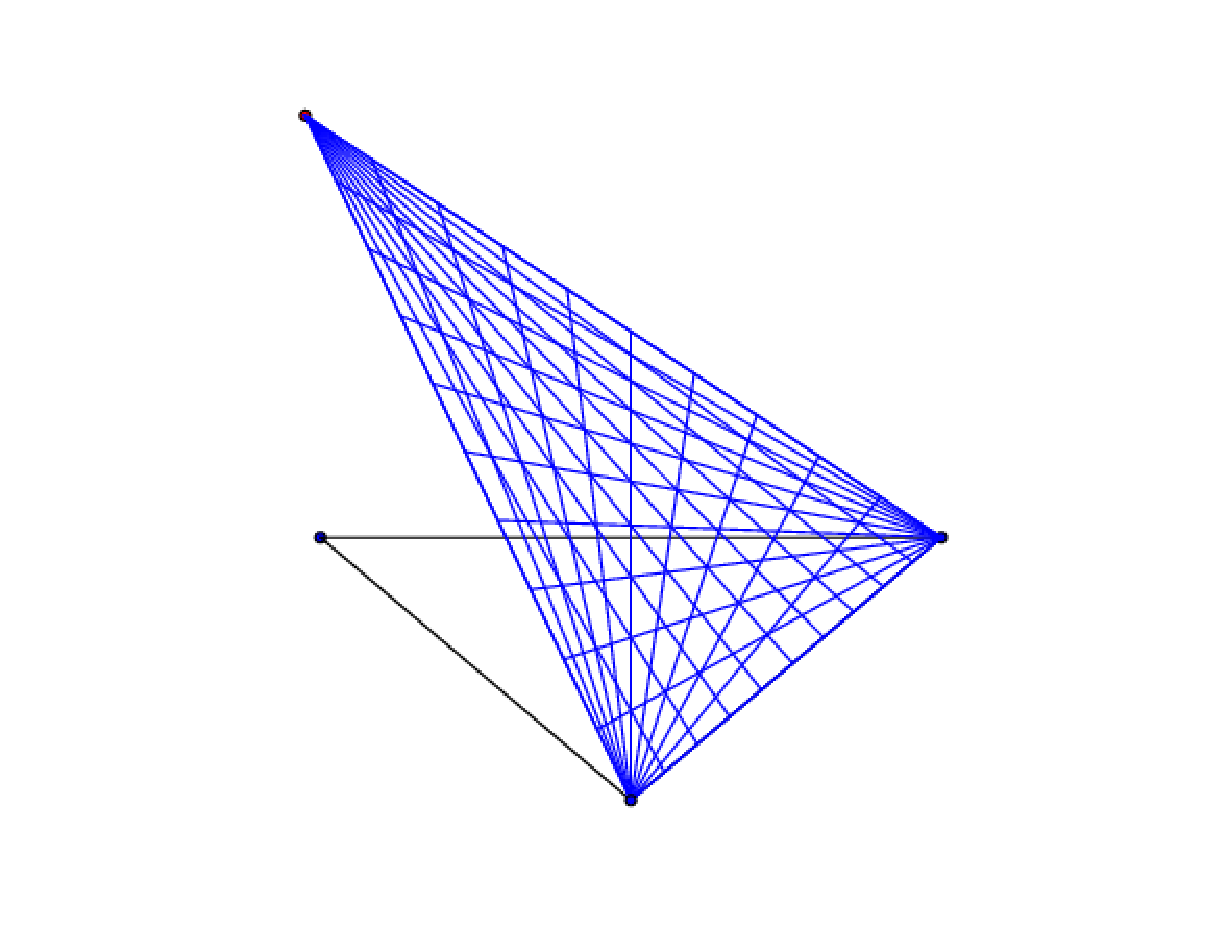
\includegraphics[width=0.6\textwidth]{images/p1_2d}
\par\end{center}

\end{frame}

\begin{frame}{Extensions: Higher dimensions}


The linear finite element method extends naturally on simplicies {[}line
elements, triangle elements, tetrahedrons{]}. Basis functions are
set to 1 at one vertex and to zero on the others. E.g. for triangles:


\begin{center}
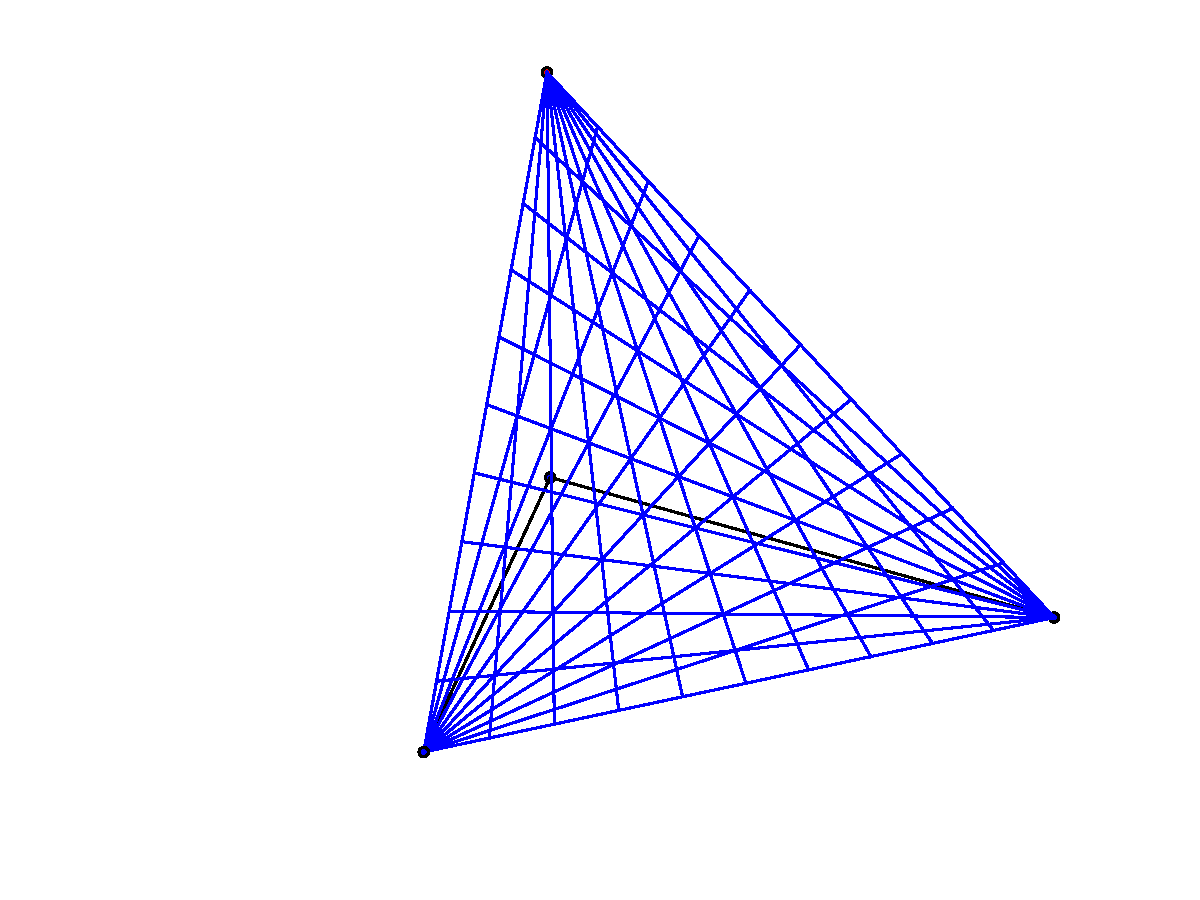
\includegraphics[width=0.6\textwidth]{images/p1_0005}
\par\end{center}

\end{frame}

\begin{frame}{Extensions: Higher dimensions}


The linear finite element method extends naturally on simplicies {[}line
elements, triangle elements, tetrahedrons{]}. Basis functions are
set to 1 at one vertex and to zero on the others. E.g. for triangles:


\begin{center}
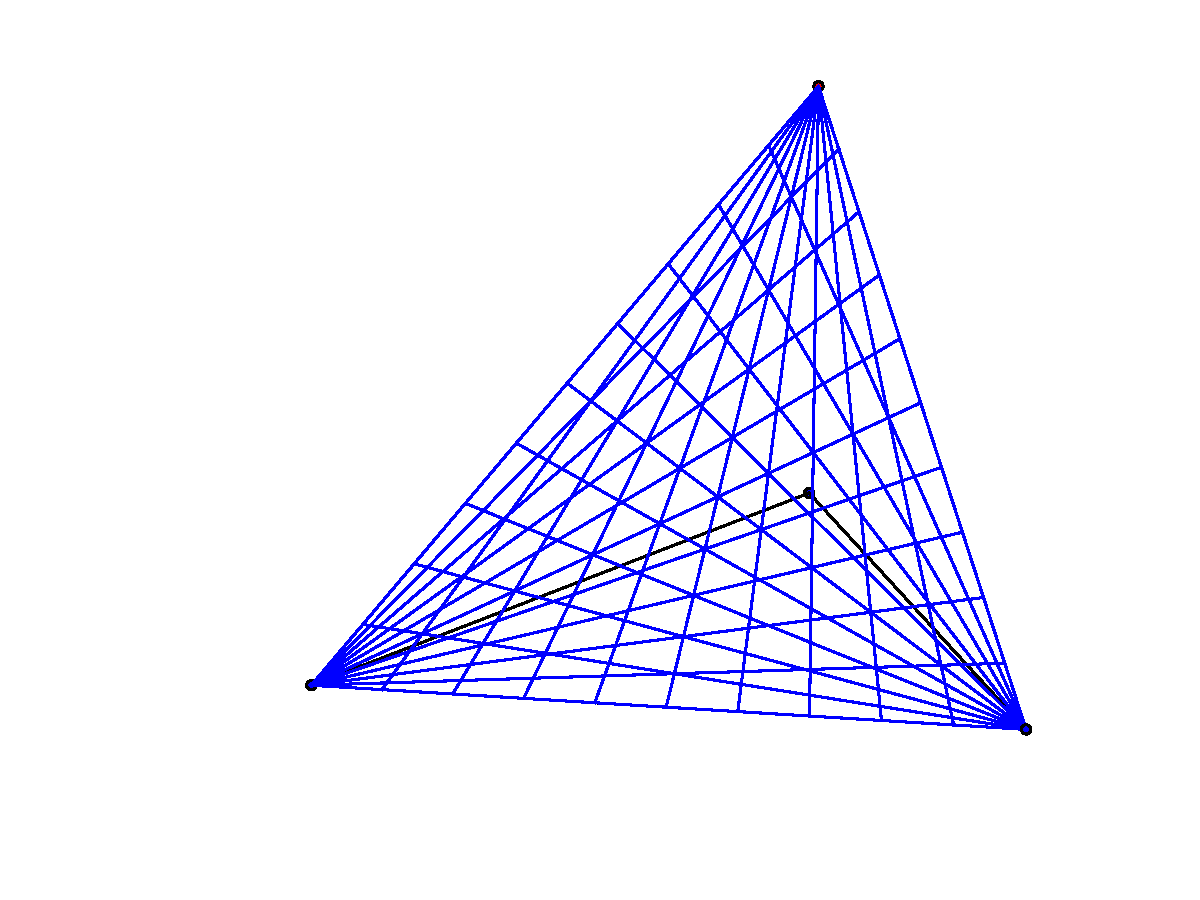
\includegraphics[width=0.6\textwidth]{images/p1_0010}
\par\end{center}

\end{frame}

\begin{frame}{Extensions: Higher dimensions}


The linear finite element method extends naturally on simplicies {[}line
elements, triangle elements, tetrahedrons{]}. Basis functions are
set to 1 at one vertex and to zero on the others. E.g. for triangles:


\begin{center}
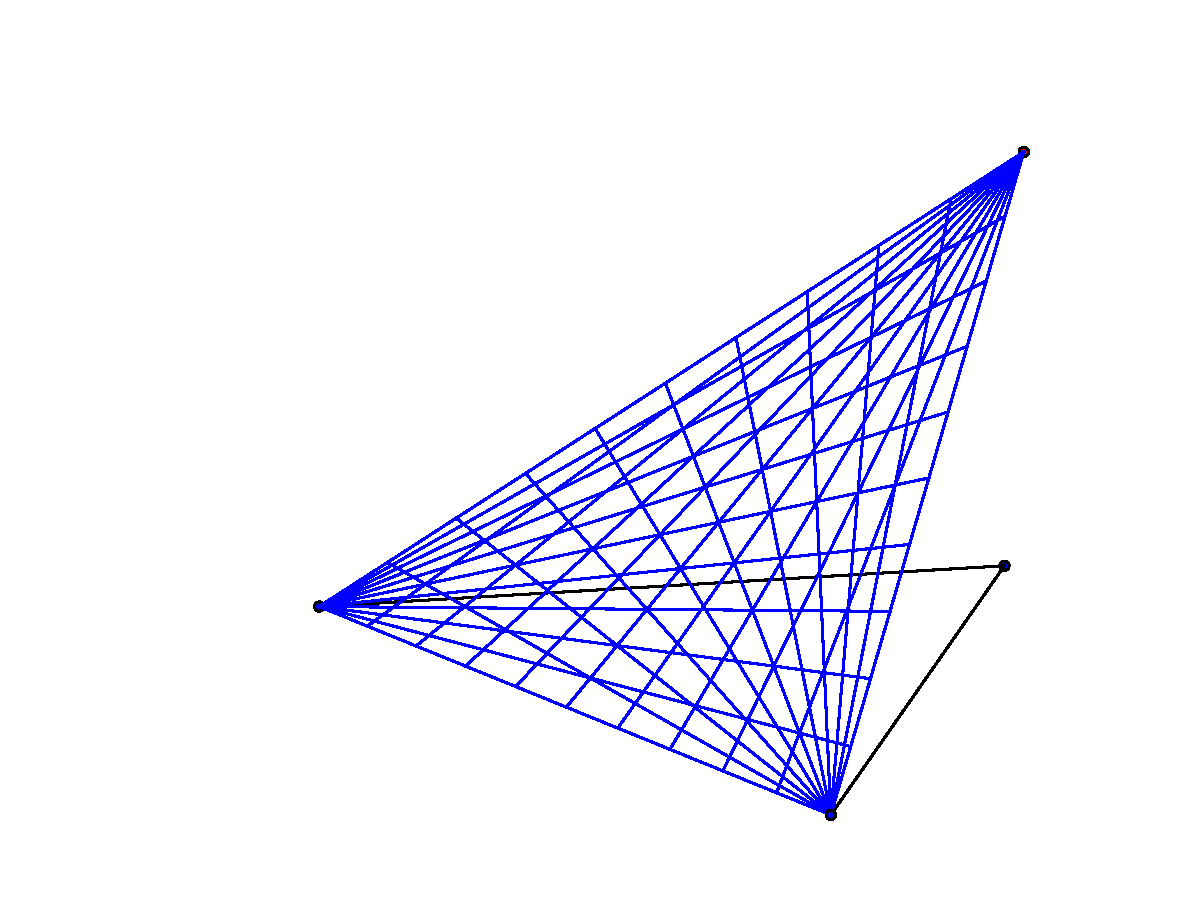
\includegraphics[width=0.6\textwidth]{images/p1_0015}
\par\end{center}

\end{frame}

\begin{frame}{ Increasing the degrees of freedom}


To increase the number of free parameters in the approximate solution
space (and thus attempt to get a more accurate solution) there are
several options:
\begin{itemize}
\item More, smaller subdivisions {[}step size,$h${]} 

\begin{itemize}
\item This is the system used in Fluidity's mesh adaptivity.
\end{itemize}
\item Use higher order polynomials, e.g. quadratic functions {[}polynomial
order, $p${]}
\item Use discontinuous functions {[}Discontinuous Galerkin formulation{]}
\end{itemize}
\end{frame}

\subsection{High order polynomials and discontinous FEM}
\begin{frame}{Increasing the degrees of freedom}

\begin{itemize}
\item Projection (in black) of smooth function (red).
\item Linear, continuous basis, Galerkin method (P1 CG).
\item In 1d degrees of freedom $\approx$ no. of elements
\end{itemize}

\begin{center}
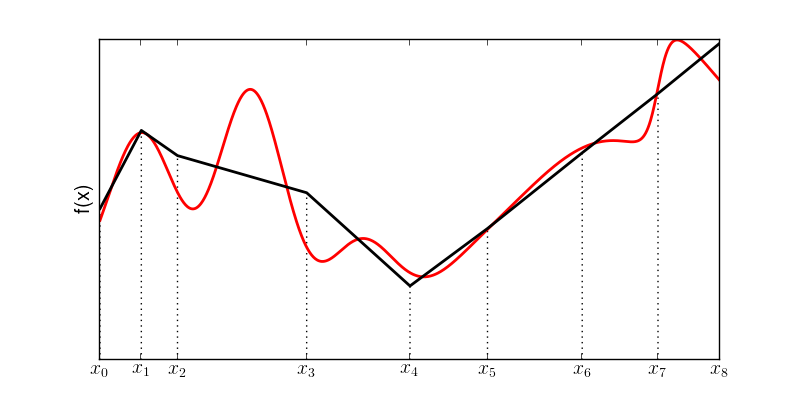
\includegraphics[width=0.9\textwidth]{images/proj_p1_low_no_err}
\par\end{center}

\end{frame}

\begin{frame}{Increasing the degrees of freedom}

\begin{itemize}
\item Projection (in black) of smooth function (red), \& error (blue).
\item Linear, continuous basis, Galerkin method (P1 CG).
\item In 1d degrees of freedom $\approx$ no. of elements
\end{itemize}

\begin{center}
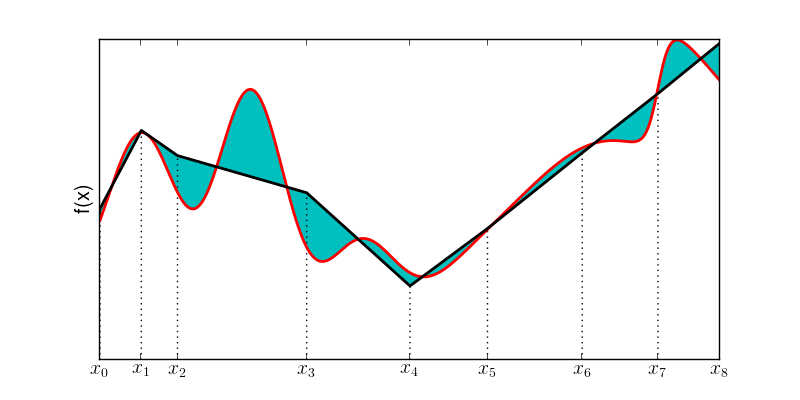
\includegraphics[width=0.9\textwidth]{images/proj_p1_low}
\par\end{center}

\end{frame}

\begin{frame}{Increasing the degrees of freedom}

\begin{itemize}
\item May increase the number of elements
\item More elements mean more degrees of freedom
\item One of the methods used in Fluidity adaptivity routines
\end{itemize}

\begin{center}
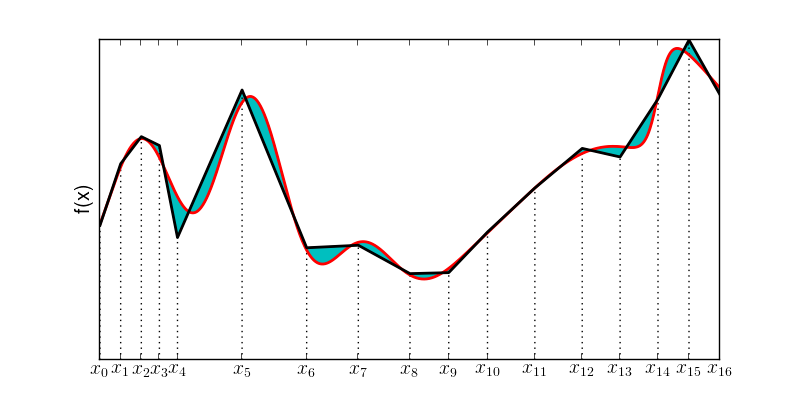
\includegraphics[width=0.9\textwidth]{images/proj_p1_high}
\par\end{center}

\end{frame}

\subsection*{Increasing the polynomial order}
\begin{frame}{Increasing the degrees of freedom}


Quadratic shape functions
\[
N_{2i}=\begin{cases}
0, & x\leq x_{i-1},\\
\frac{2x^{2}-\left(3x_{i-1}+x_{i}\right)x+\left(x_{i}+x_{i-1}\right)x_{i-1}}{\left(x_{i}-x_{i-1}\right)^{2}}, & x_{i-1}<x\leq x_{i},\\
\frac{2x^{2}-\left(3x_{i+1}+x_{i}\right)x+\left(x_{i}+x_{i+1}\right)x_{i+1}}{\left(x_{i+1}-x_{i}\right)^{2}}, & x_{i}<x\leq x_{i+1},\\
0. & x>x_{i+1}.
\end{cases}
\]
\[
N_{2i+1}=\begin{cases}
0, & x<x_{i},\\
-\frac{x^{2}-\left(x_{i+1}+x_{i}\right)x+x_{i}x_{i+1}}{\left(x_{i+1}-x_{i}\right)^{2}}, & x_{i}<x\leq x_{i+1},\\
0. & x>x_{i+\text{1}}.
\end{cases}
\]


\end{frame}

\begin{frame}{Finite Element Functions}


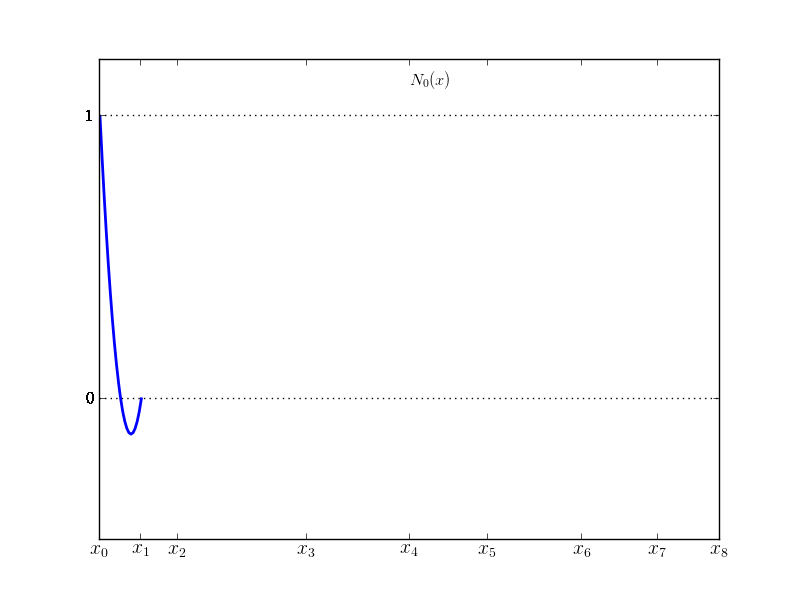
\includegraphics[width=1\textwidth]{images/N2_0}

\end{frame}

\begin{frame}{Finite Element Functions}


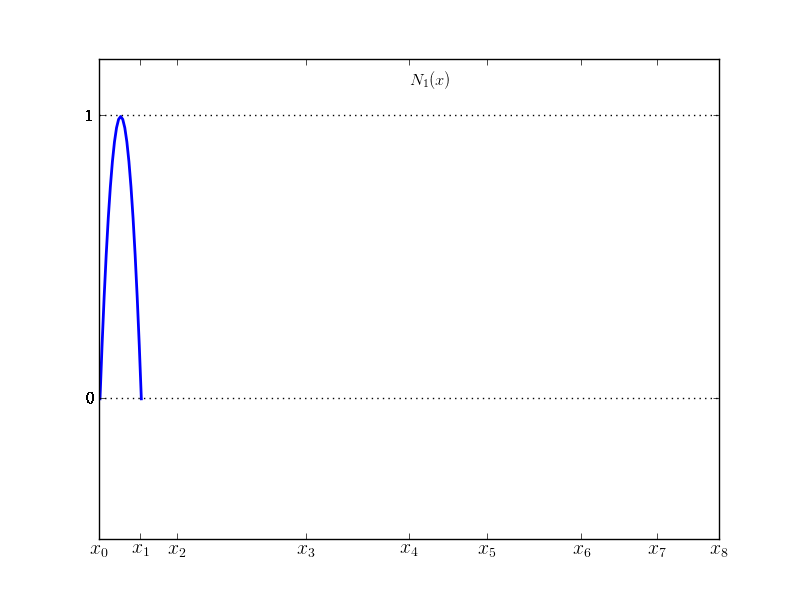
\includegraphics[width=1\textwidth]{images/N2_1}

\end{frame}

\begin{frame}{Finite Element Functions}


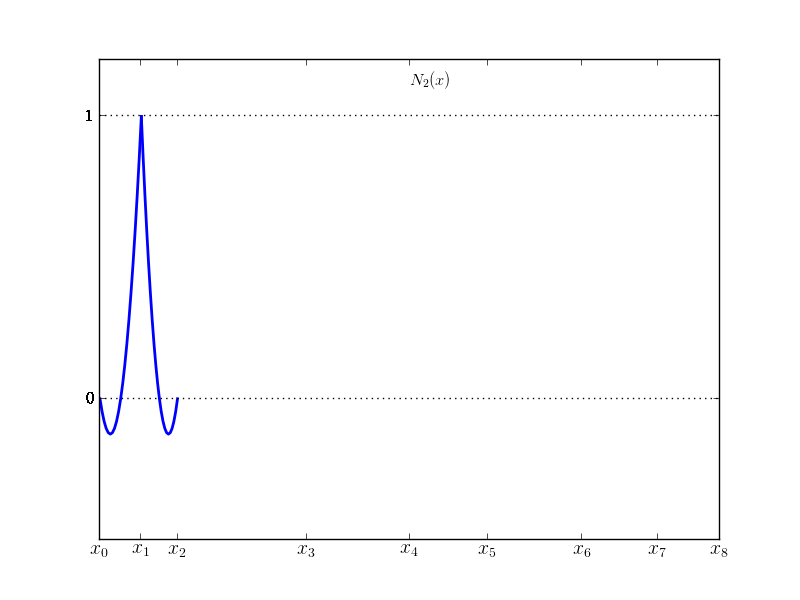
\includegraphics[width=1\textwidth]{images/N2_2}

\end{frame}

\begin{frame}{Finite Element Functions}


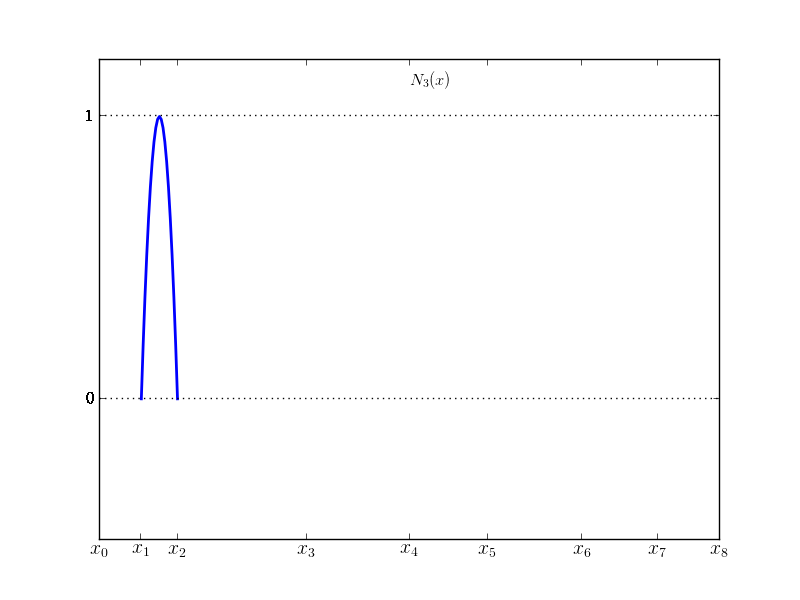
\includegraphics[width=1\textwidth]{images/N2_3}

\end{frame}

\begin{frame}{Finite Element Functions}


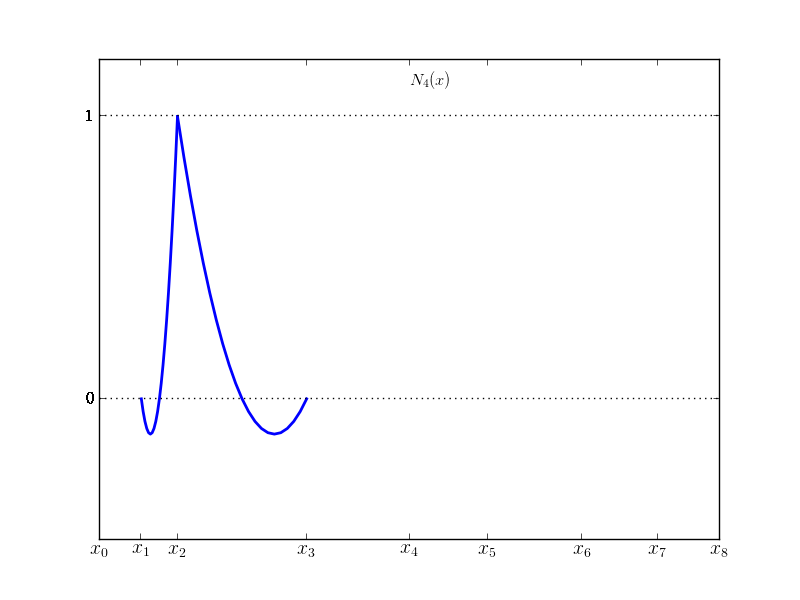
\includegraphics[width=1\textwidth]{images/N2_4}

\end{frame}

\begin{frame}{Increasing the degrees of freedom}

\begin{itemize}
\item Projection of a smooth function.
\item Quadratic, continuous basis, Galerkin method (P2 CG).
\item In 1d degrees of freedom $\approx$ 2 $\times$ no. of elements.
\item Good representation of slowly varying functions
\end{itemize}

\begin{center}
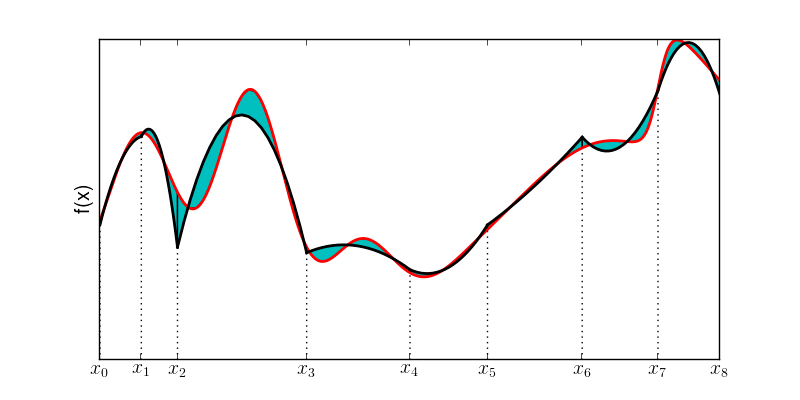
\includegraphics[width=0.9\textwidth]{images/proj_p2}
\par\end{center}

\end{frame}

\subsection*{Discontinuous elements}
\begin{frame}{Increasing the degrees of freedom}


Discontinuous linear shape functions
\[
N_{2i}=\begin{cases}
0, & x\leq x_{i},\\
\frac{\left(x_{i+1}-x\right)}{\left(x_{i+1}-x_{i}\right)}, & x_{i}<x\leq x_{i+1},\\
0. & x>x_{i+1}.
\end{cases}
\]
\[
N_{2i+1}=\begin{cases}
0, & x<x_{i},\\
-\frac{\left(x-x_{i}\right)}{\left(x_{i+1}-x_{i}\right)}, & x_{i}<x\leq x_{i+1},\\
0. & x>x_{i+\text{1}}.
\end{cases}
\]


\end{frame}

\begin{frame}{Increasing the degrees of freedom}

\begin{itemize}
\item Projection of a smooth function.
\item Linear, discontinuous basis, Galerkin method (P1 DG).
\item In 1d degrees of freedom $\approx$2 \textrm{$\times$} no. of elements.
\item Good representation of discontinuties/fronts/large gradients.
\end{itemize}

\begin{center}
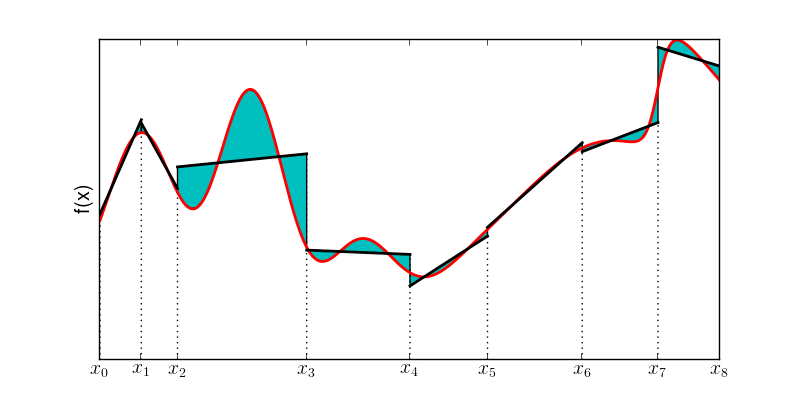
\includegraphics[width=0.9\textwidth]{images/proj_p1_dg}
\par\end{center}

\end{frame}

\begin{frame}{Review of Section}

\begin{itemize}
\item The degrees of freedom (and thus size) of a problem can be increased
by:

\begin{itemize}
\item increasing the number of element subdivisions (making step size $h$
smaller)
\item increasing the order of the shape functions applied on elements (increasing
polynomial degree, $p$)
\item relaxing continuity constraints at the interface between elements
(discontinuous Galerkin method, nonconforming elements)
\end{itemize}
\end{itemize}
\end{frame}

\section{Spaces, Forms and Functions\label{sec:SFF}}


\subsection{More on Vector Spaces}
\begin{frame}{Reassuring Mathematics}


This section summarises some useful results from mathematical analysis
for finite element problems. In particular, we note that results exists
to show that, under certain provisos finite element solutions to a
given problem
\begin{itemize}
\item exist
\item are unique
\item converge
\item converge to the right answer.
\end{itemize}
\end{frame}

\begin{frame}{Choice of Vector Spaces}


Going back to the weak form for the original infinite dimensional
problem,
\[
\int_{\Omega}\nabla\phi\cdot\nabla\psi\: dV=\int_{\Omega}\phi f\: dV+\int_{\delta\Omega^{N}}\phi b\: dV,
\]
it is obvious that $\psi$ and $\nabla\psi$ must be well behaved
enough for these integrals to exist. 

\end{frame}

\begin{frame}{Choice of Vector Spaces}


We require the function is square integrable,
\begin{equation}
\left\Vert \psi\right\Vert ^{2}:=\int_{\Omega}\psi^{2}\: dV<\infty.
\end{equation}
(The space of function which satisfy this is normally called $\mathcal{L}_{2}\left(\Omega\right)$)
and also that
\begin{equation}
\left\Vert \nabla\psi\right\Vert ^{2}:=\int_{\Omega}\nabla\psi\cdot\nabla\psi\: dV<\infty,
\end{equation}
Functions which satisfy both (1) \& (2) are in the space of square
integrable functions with square integrable derivatives, denoted $\mathcal{H}^{1}\left(\Omega\right)$.
This is a \emph{Sobolev space}.

\end{frame}

\begin{frame}{Weak equations and Bilinear forms}


The volume integral in ({*}) defines a symmetric bilinear form, $a:\mathcal{H}^{1}\left(\Omega\right)\times\mathcal{H}^{1}\left(\Omega\right)\rightarrow\mathbb{R},$
\[
a(\phi,\psi):=\int_{\Omega}\nabla\psi\cdot\nabla\phi\: d^{n}x.
\]



where
\begin{alignat*}{1}
a\left(\phi,\psi\right) & =a\left(\psi,\phi\right),\\
a\left(c_{1}\phi+c_{2}\xi,\psi\right) & =c_{1}a\left(\phi,\psi\right)+c_{2}a\left(\xi,\psi\right).
\end{alignat*}


\end{frame}

\begin{frame}{Lax-Milgram Theorem}


Two properties of the bilinear form, $a$, are used to show well-posedness:
\[
\tag{continuity }a(\phi,\psi)\leq C\left\Vert \psi\right\Vert \left\Vert \phi\right\Vert \mbox{ for some C}>0,
\]
\[
\tag{coercive/elliptic}a(\psi,\psi)\geq c\left\Vert \psi\right\Vert ^{2}\mbox{ for some c>0.}
\]


\end{frame}

\subsection{Existence, Uniqueness and Convergence of Solutions}
\begin{frame}{Well posedness - existence }


Existence follows from application of Riesz representation theorem
to the Hilbert space problem
\[
a\left(u,v\right)=f\left(v\right),
\]
Precise details lie outside of the scope of this lecture, but effectively
guarantees an ``inverse'' to the map
\[
\phi_{v}\left(u\right)=a\left(u,v\right),
\]
so that for sufficiently smooth data we can always get a solution.

\end{frame}

\begin{frame}{Well posedness - uniqueness:}


Suppose there are two different solutions, $\psi_{1}$ and $\psi_{2}$,
i.e.


\[
a\left(\phi,\psi_{1}\right)=a\left(\phi,\psi_{2}\right)=\int_{\Omega}\phi f\, d^{n}x,\mbox{ for all }\phi\in\mathcal{H}^{1}\left(\Omega\right).
\]
Then
\[
a\left(\phi,\psi_{1}-\psi_{2}\right)=0
\]
but $\psi_{1}-\psi_{2}\in\mathcal{H}^{1}\left(\Omega\right),$ so
can choose to test $\phi=\psi_{1}-\psi_{2}$ Then
\[
a\left(\psi_{1}-\psi_{2},\psi_{1}-\psi_{2}\right)=0\geq c\left\Vert \psi_{1}-\psi_{2}\right\Vert ^{2},
\]
So $\psi_{1}=\psi_{2},$ hence solution is unique.

\end{frame}

\begin{frame}{Well posedness - convergence}


Let $\psi\in\mathcal{V}$ be exact solution, $\psi^{\delta}\in\mathcal{V}^{\delta}\subset\mathcal{V}$
be the finite element solution $\xi\in\mathcal{V}^{\delta}$ be an
arbitrary function. Then $\psi^{\delta}-\xi\in\mathcal{V}$ and $\psi^{\delta}-\xi\in\mathcal{V}^{\delta}$
and 
\[
\tag{From PDE}a(\underbrace{\psi^{\delta}-\xi}_{\in\mathcal{V}},\psi)=\int_{\Omega}\left(\psi^{\delta}-\xi\right)fd^{n}x
\]
\[
\tag{FEM}a(\underbrace{\psi^{\delta}-\xi}_{\in\mathcal{V^{\delta}}},\psi^{\delta})=\int_{\Omega}\left(\psi^{\delta}-\xi\right)fd^{n}x
\]


\end{frame}

\begin{frame}{Well posedness - convergence}


\begin{align*}
c\left\Vert \psi-\psi^{\delta}\right\Vert ^{2}\leq & a\left(\psi-\psi^{\delta},\psi-\psi^{\delta}\right),\\
 & =a\left(\psi-\psi^{\delta},\psi-\psi^{\delta})+a(\psi-\psi^{\delta},\psi^{\delta}-\xi\right)\\
 & \qquad\qquad+a\left(\psi^{\delta}-\xi,\psi^{\delta}\right)-a\left(\psi^{\delta}-\xi,\psi\right),\\
 & =a\left(\psi-\psi^{\delta},\psi-\psi^{\delta}+\psi^{\delta}-\xi\right)\\
 & \qquad\qquad-\int_{\Omega}\left(\psi^{\delta}-\xi\right)fd^{n}x+\int_{\Omega}\left(\psi^{\delta}-\xi\right)fd^{n}x,\\
 & =a\left(\psi-\psi^{\delta},\psi-\xi\right)\leq C\left\Vert \psi-\psi^{\delta}\right\Vert \left\Vert \psi-\xi\right\Vert .
\end{align*}


\end{frame}

\begin{frame}{Well posedness - convergence}


Hence it is guaranteed (Cea's lemma)
\[
\left\Vert \psi-\psi^{\delta}\right\Vert \leq\frac{C}{c}\inf_{\xi\in\mathcal{V}^{\delta}}\left\Vert \psi-\xi\right\Vert .
\]
Choose $\xi$ to be linear projection of $\psi$, i.e $\xi\left(x_{i}\right)=\psi\left(x_{i}\right),$
$\frac{\partial^{2}\xi}{\partial x^{2}}=0$, then
\[
\left\Vert \psi-P\psi\right\Vert \leq\alpha\sup_{\Omega_{i}}h_{i}\sup_{x\in\Omega}\left|\frac{\partial^{2}\psi}{\partial x^{2}}\right|
\]
Hence
\[
\left\Vert \psi-\psi^{\delta}\right\Vert \leq\frac{\alpha C}{c}\sup_{\Omega_{i}}h_{i}\sup_{x\in\Omega}\left|\frac{\partial^{2}\psi}{\partial x^{2}}\right|
\]
\[
\left\Vert \psi-\psi^{\delta}\right\Vert \rightarrow0\mbox{ as }\sup_{\Omega_{i}}h_{i}\rightarrow0.
\]


\end{frame}

\begin{frame}{Review of Section}


We have shown that finite element approximations to the solutions
to PDEs
\begin{itemize}
\item are unique,
\item converge,
\item and converge to the right answer.
\end{itemize}

We have also given a hint that they exist. We have also shown that
by using knowledge about the form of the solution we can choose elements
to minimize the estimated error for a given number of degrees of freedom.

\end{frame}

\section{A Note on Implementation}
\begin{frame}{Quadrature}


Numerical method to calculate/approximate integrals:


\[
\int_{a}^{b}f\left(\bm{x}\right)d^{n}x\approx\sum_{x=1}^{N}w_{i}f\left(\bm{p}_{i}\right)
\]



\begin{center}
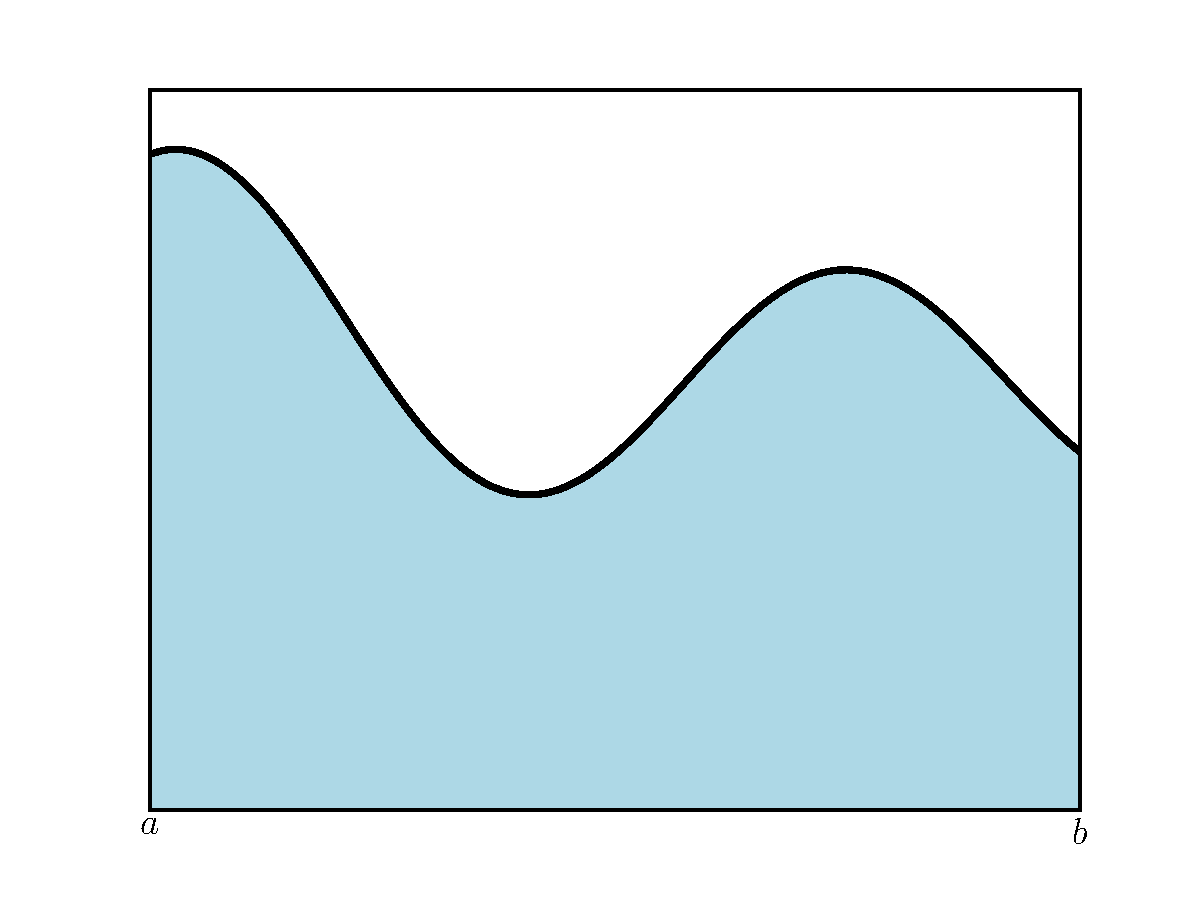
\includegraphics[bb=0bp 20bp 576bp 412bp,width=0.7\textwidth]{images/quad_func_0}
\par\end{center}

\end{frame}

\begin{frame}{Quadrature}


Numerical method to calculate/approximate integrals:


\[
\int_{a}^{b}f\left(\bm{x}\right)d^{n}x\approx\sum_{x=1}^{N}w_{i}f\left(\bm{p}_{i}\right)
\]



\begin{center}
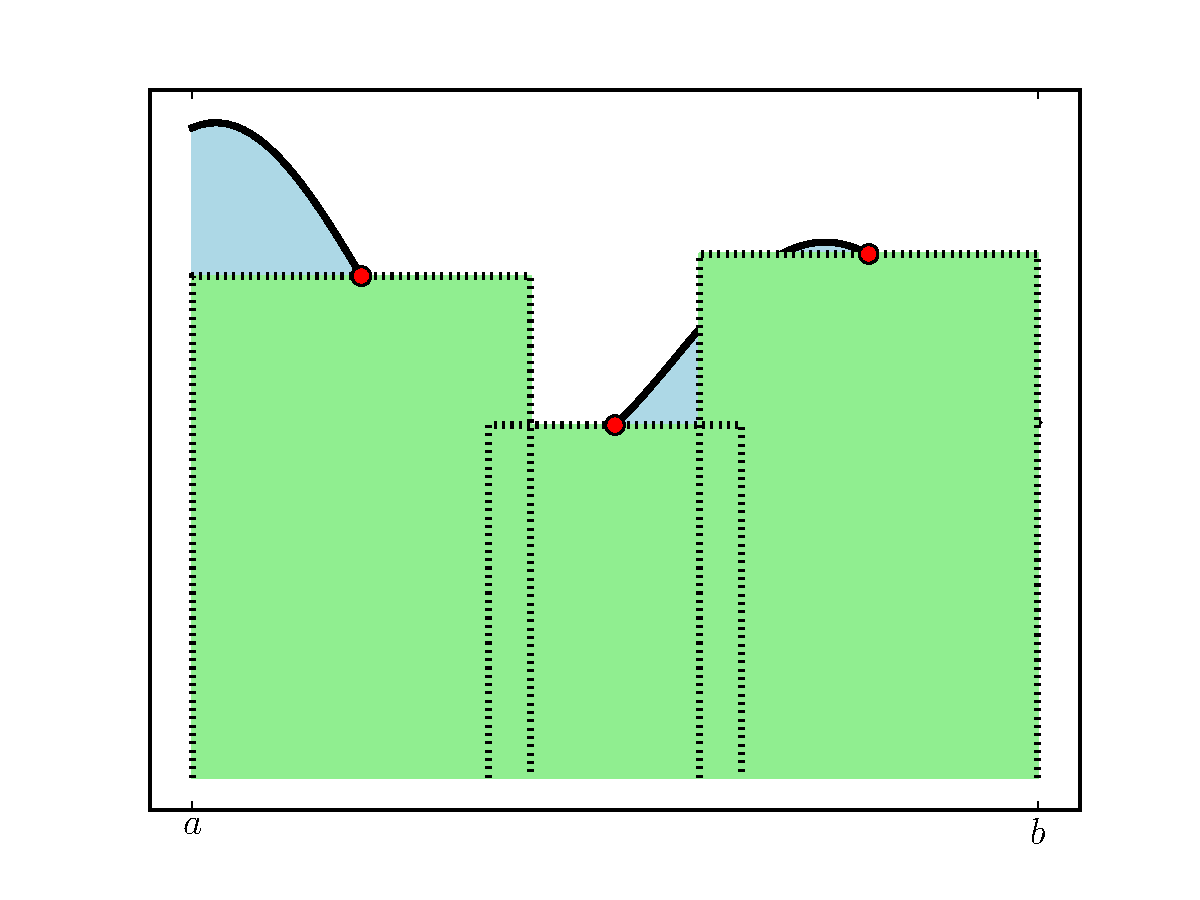
\includegraphics[bb=0bp 20bp 576bp 412bp,width=0.7\textwidth]{images/quad_func_1}
\par\end{center}

\end{frame}

\begin{frame}{Quadrature}


Some famous quadratures:
\begin{enumerate}
\item Midpoint rule {[}one point method{]}
\[
w=a-b,\quad p=\frac{a+b}{2},
\]

\item Simpson's rule {[}3 point method{]}
\[
w_{1}=\frac{a-b}{6},\quad w_{2}=\frac{4\left(a-b\right)}{6},\quad w_{3}=\frac{a-b}{6},
\]
\[
p_{1}=a,\quad p_{2}=\frac{a+b}{2},\quad p_{3}=b,
\]

\end{enumerate}
\end{frame}

\begin{frame}{Quadrature}


The degree or order of a quadrature rule over an interval is the largest
integer, n such that method is exact for all
\[
p_{n}=a_{0}x^{n}+a_{1}x^{n-1}+\ldots a_{n}\quad a_{i}\in\mathbb{R}.
\]


\end{frame}



\section*{Summary}
\begin{frame}{Summary}

\begin{itemize}
\item Finite element methods solve a \emph{weak form} of the \emph{exact}
equations in an \emph{approximate solution space}.
\item The approximate \emph{solution} is defined (almost) \emph{everywhere}.
\item \emph{Neuman conditions} dealt with implicitly inside formulation
\item \emph{Dirichlet conditions} appear in right hand side (as in finite
difference methods).
\end{itemize}
\end{frame}
\appendix

\section*{Appendix}


\subsection*{Useful References}
\begin{frame}{References}


\beamertemplatebookbibitems
\begin{thebibliography}{References}
\bibitem{Author1990}J. Donea \& A. Huerta \newblock Finite Elements
Methods for Flow Problems.\newblock Wiley 2003

\bibitem{Reddy} J.N. Reddy \& D.K. Gartling\newblock The Finite
Element Method in Heat Transfer and Fluid Dynamics\newblock CRC Press
1994\beamertemplatearticlebibitems

\bibitem{key-2}Fluidity Manual\newblock AMCG\newblock 2014\end{thebibliography}
\end{frame}

\end{document}
